% Created 2010-05-31 Mon 17:03
\documentclass[11pt]{article}
\usepackage[utf8]{inputenc}
\usepackage[T1]{fontenc}
\usepackage{graphicx}
\usepackage{longtable}
\usepackage{float}
\usepackage{wrapfig}
\usepackage{soul}
\usepackage{amssymb}
\usepackage{hyperref}
\usepackage[top=3cm, bottom=3cm, left=2cm, right=2cm]{geometry}

\title{inf1050-notater}
%\author{Sjur Hernes}
\date{31 May 2010}

\begin{document}

\maketitle

\setcounter{tocdepth}{3}
\tableofcontents
\vspace*{1cm}
\section{Kapittel 1 - Hva er programvare?}
\label{sec-1}
\subsection{Introduksjon}
\label{sec-1.1}

  Programvare brukes over alt i dagens samfunn. Har ingen direkte fysisk begrensing, 
  og kan derfor fort bli svært komplekst og uoversiktelig. Prisantydning kan være 
  vanskelig og prosjekter slår ofte feil og overskrider budsjettet. Software Enginering 
  prøver å endre dette ved å gi verktøy for prosjektanalyse etc. 
\subsection{Hva er programvare?}
\label{sec-1.2}

\begin{itemize}
\item Software (en samling programmer og tilhørende dokumentasjon etc.).
     Vi har govt sett to typer:

\begin{enumerate}
\item Standard konsumer-programvare.
\item Kustomisert programvare (spesialdesignet for ett firma etc.)
\end{enumerate}

\end{itemize}

  Fem viktige attributter til god programvare: 
\begin{itemize}
\item God, forståelig kode for senere forbedringer.
\item Stabil
\item sikker og fortrolig programvare.
\item Effektiv.
\item Brukervennlig.
\end{itemize}
\subsection{Hva er systemutvikling?}
\label{sec-1.3}

\begin{itemize}
\item Systematisk og organisert fremgangsmåte. 
     Tar også hensyn til organisatorisk og økonomiske begrensninger i prosessen.
\end{itemize}
  
   På grunn av stor innvirkning av samfunnet er software engineers nødt til å opptre etisk og tenke konsekvenser. 

   Software engineering er et tverrfaglig foretagende!

   Baserer seg på de systematiske ingeniørprinsippene:
\begin{itemize}
\item Planlegging og forutsigbarhet
\item Oppdeling og strukturering av problemer i mindre komplekse bestanddeler
\item Modularitet og gjenbruk
\item Abstraksjon og modellering
\item Systematisk kvalitetssikring
\end{itemize}

   En enkel oppdeling og strukturering av prosessen kan se slik ut:
\begin{itemize}
\item Tid (faser):

\begin{itemize}
\item PS2000-kontraktstandarden: Behovsfase, Løsningsbeskrivelse, Iterativ konstruksjonsfase, Godkjenningsfase.
\item Timeboxing/tidsavgrensning.
\end{itemize}

\item Oppgaver (aktiviteter og tilhørende leveranser):

\begin{itemize}
\item Analyse, design, programmering, testing,\ldots{}
\end{itemize}

\item Tekniske aspekter:

\begin{itemize}
\item Kvalitetsaspekter, Funksjonalitet, Moduler, Komponenter.
\end{itemize}

\item Modeller på forskjellige abstraksjonsnivåer

\begin{itemize}
\item Kravspesifikasjoner versus Objektorientert analyse versus Detaljert design versus Kode.
\end{itemize}

\end{itemize}
\section{Kapittel 2 - Sosiotekniske systemer}
\label{sec-2}


  Et sosio-teknisk system består av mer enn bare programvare (maskinvare, mennesker).

  Et system er en sammensetning av komponenter som sammen jobber mot et mål.
\subsection{Definisjon teknisk system}
\label{sec-2.1}

   Et teknisk system er systemer som inneholder både programvare og maskinvare, men prosedyrer eller prosesser. 
\subsection{Definisjon Sosio-teknisk system}
\label{sec-2.2}

   Et sosio-teknisk system inneholder i tillegg operatører som har kunnskap om hvordan systemet skal brukes. 
   (Karakteristikker er, ikke-deterministisk output ved lik input, 
\subsection{Om systemer}
\label{sec-2.3}


   Et system er en sammensetning av flere deler som virker sammen. Ikke enkeltkomponenter, men samspillet.
   Eksempler: Fly, biler, bankterminaler, etc.

   Typer av egenskaper: Funksjonelle og ikke-funksjonelle egenskaper. Altså være et transportmiddel (funksjonell)
   eller sikker, pålitelig, ytelse, etc (ikke-funksjonell).

   Et system har tre punkter som avgjør pålitligheten:
  
\begin{enumerate}
\item Hardware-feil.
\item Software-feil.
\item Operatørfeil.
\end{enumerate}

   Sikkerheten til et system er det vanskeligste å anta. Man vet aldri om et system er helt sikkert, kun når det ikke er sikkert.
\subsection{Systemutvikling}
\label{sec-2.4}


   Systemutvikling gjelder for spesifisering, design, implementering, validering, iverksette og 
   vedlikeholde sosio-tekniske systemer. Siden mange utviklingsavgjørelser gjøres på grunnlag av 
   systemutviklingsprosessen er det også viktig at utviklerene vet om prosessen.
\subsubsection{Vi har tre former for system-krav}
\label{sec-2.4.1}

\begin{enumerate}
\item Abstrakte funksjonskrav: Basisfunksjonene til systemet.
\item Sysem-egenskaper: De ikke-funksjonelle kravene.
\item Hva systemet ikke må gjøre.
\end{enumerate}
\subsubsection{Systemmodelering}
\label{sec-2.4.2}

    Deler opp systemet i sub-systemer og ser på avhengighetsforhold. 
    Sub-systemene kan så igjen være nye uavhengige systemer, eller komponenter man henter inn.
    I systemintegreringsprosessen tar du alle de uavhengig utviklede sub-systemene og setter
    sammen til et komplett system. Pleier å gjøres inkrementelt. (sub-systemene er sjeldent 
    ferdig samtidig og gjør feilsøking letter og billigere).
\subsubsection{System-evolsjon}
\label{sec-2.4.3}

    Det gjøres etterhvert endringer i systemer, både hardware og funksjons/software-messig. 
    Dette blir etterhvert dyrere, og man må være forsiktig, siden det kan oppstå problemer med sub-systemene og hvordan de spiller sammen.
\subsubsection{System-dekomponering}
\label{sec-2.4.4}

    Hardware-messig kan det bety å pakke sammen utstyr og sende til gjenvinning.
    Software kan bety å hente ut verdifull data, til en ny database etc.
\subsubsection{Større systemer}
\label{sec-2.4.5}

    På større systemer har man ikke mulighet til å gjøre hele system-utviklingsprosessen selv, og man setter 
    ut f.eks. deler av sub-systemene på anbud.
\subsection{Rammer}
\label{sec-2.5}

   Menneskelige, politiske og organisatoriske bestemmelser har en stor effekt på sosio-tekniske systemer.
\section{Kapittel 3 - Kritiske systemer}
\label{sec-3}

  Kostnadene for kritiske systemer er MYE høyere. 
  Må gjennomgå mye dyr testing og bevisføring av systemet og koden.
  Det er også mye mer som står på spill om noe galt skulle skje, både økonomiske skader og menneskelige skader.

  Den mest viktige emergens-egenskapen til et kritisk system er pålitelighet 
  (som igjen kan bestå av tilgjengelighet (at den på ett gitt punkt faktisk svarer 
  deg på forespørsel), reliability (sannsynlighet for at systemet fungerer), 
  sikkerhet (safety) og sikkerhet (security). 
\subsection{Sikkerhets-kritiske systemer:}
\label{sec-3.1}

   Kan resultere i skade, tap av liv eller miljøskader.
\subsection{Oppgave-kritiske systemer:}
\label{sec-3.2}

   Feil gjør at hovedoppgaven feiler. F.eks. styringssystem til fly.
\subsection{Business-kritiske systemer:}
\label{sec-3.3}

   Fører til store økonomiske skader for bedriften.
\subsection{De tre hovedårsakene til feil}
\label{sec-3.4}

\begin{enumerate}
\item hardware-feil
\item feil i spesifiseringen av systemet
\item operatør-feil.
\end{enumerate}

   Må ta hensyn til menneskene som er med i systemet, samt alle komponentene som jobber sammen.
\subsubsection{Faser i en livssyklus}
\label{sec-4.1}


\begin{enumerate}
\item Idefase om et system – foretningsanalyse (lønner det seg)
\item Kravinnsamling og kravanalyse (hva skal systemet gjøre?)
\item Design (hvordan skal det konstrueres?)
\item Programmering (konstruksjon)
\item Test (ble det riktig?)
\item Installasjon, integrasjon, driftsetting
\item Vedlikehold (feilretting og videreutvikling)
\end{enumerate}
\section{Kapittel 4 - Systemutviklingsprosess}
\label{sec-4}

  Hvordan programvare skal produseres. Organiseringen rundt det å skrive kode etc.
  76\% av alle prosjekter overskrider budsjett. 19\% bruker mindre.
  Økt produktivitet og kvalitet.
\subsection{Utviklingsmodeller.}
\label{sec-4.1}

     
   Store kostnader med utvikling av systemer og dermed har man over
   tid fått mange forskjellige utviklingsmodeller som kan hjelpe oss
   å minimere risiko og kostnad for utviklingen.
\subsubsection{Fossefallsmodellen:}
\label{sec-4.1.1}

\begin{enumerate}
\item Requirements analysis and definition: 
      Tjenester og mål for systemet defineres, etter samtaler med bruker.
\item System and software design: 
      Beskriver system-arkitekturen.
\item Implementation and unit testing: 
      Sjekker hver komponent om de går sammen etc.
\item Integration and unit testing: 
      Komponenter settes sammen og testes som et system. Krav sjekkes. Leveres!
\item Operation and maintanane: 
      Systemet innstaleres, og eventuelle usette feil rettes,nye krav oppdages og legges til.
\end{enumerate}

   Gjør få iterasjoner. Fasene avsluttes for ny startes. Dyrt med endringer.
   Kun når kravene er meget godt definert, og man føler seg sikker på prosessen.
\subsubsection{Evoutionary development:}
\label{sec-4.1.2}

    Kommer med raske utkast, viser dem til kunden og får tilbakemeldinger og gjør endringer. Dette gjøres til resultatet er akkseptabelt.

\begin{enumerate}
\item Exploratory develpoment: 
       Vidreutvikler de delene man forstår, har samtaler underveis.
\item Throwaway prototyping: 
       Eksperimenterer med de dårlig forståtte kravene, og kaster det.
\end{enumerate}

    Problemer: Litt vanskelig for ledere å vite lengde, estimere etc. 
    Samt at systemet blir dårligere strukturert når man bare legger til og legger til. 

    En kombinasjon av evolusjonær og fossefall kan være bra. Definere krav med evo. og fossefall på de godt forståtte delene.
\subsubsection{Component based software engineering:}
\label{sec-4.1.3}

    Tar sikte på å gjenbruke komponenter. 
    
\begin{enumerate}
\item Component analysis: 
       Ser på krav, og leter etter komponenter. Passer ikke alltids nødvendigvis.
\item Requirements modifications: 
       Ser på kravene igjen i forhold til kompoonenter. 
       Endrer på kravene hvis det lar seg gjøre. Hvis ikke letes det etter nye komponenter.
\item System design with reuse: 
       Framework settes sammen. Noen komponenter må kanskje designes, hvis det ikke finnes noe å gjenbruke.
\item Development and integration: 
       Noe kode kan måtte skrives her. Systemet settes så sammen.
\end{enumerate}

    Billigere med gjennbruk, prosessen kan gå raskere, men kompromisser på alltids gjøres i forhold til kravene.
\subsubsection{Process iteration:}
\label{sec-4.1.4}

    Kravene forandrer seg stort under en prosess. Ny teknologi, press utenfra, forandring i ledelse etc. 
    Inkrementelle prosesser prøver å ta forbehold om dette.
\begin{itemize}
\item Systemspesifikasjonene er ikke ferdig før siste inkrement er ferdig.
\end{itemize}
\subsubsection{Incremental delivery:}
\label{sec-4.1.5}

    Skriver generelle outline-krav og struktur. Så skriver man krav til enkeltinkrementer, utvikler dem og leverer deler, og skriver nye krav til nye inkrementer.
\begin{enumerate}
\item Fordeler: 
      Kan få ett fungerende system tidlig. Mest kritisk uvikles først. 
      Kan ut fra erfaring forme nye krav til inkrement. Lavere risiko for total prosjekt-kolaps.
\item Spiral development: 
      Utviklingsfasen er illustrert i en sipral som går utover.
\item Objective setting: 
       Formål med fasen settes. Risiko settes.
\item Risk assesment and redction: 
       Analyse av risk blir gjort. Nødvendig handling utføres.
\item Development and validation: 
       Utviklingsmodell velges. Fossefall, inkrementell, evolusjonær etc.
\item Planning: 
       Prosjektet evalueres og man ser om det er nødvendig å gå en spiral til.
\end{enumerate}
\subsubsection{Process activites}
\label{sec-4.1.6}
\begin{itemize}

\item Software specification:\\
\label{sec-4.1.6.1}%
\begin{enumerate}
\item Feasibility study: 
       Ser om det er mulig å utvikle, om det er lønnsomt og om det kan gjøres innenfor budsjett. 
       Gjøres raskt. Gir klarsignal for vidre arbeid.
\item Requirements elicitation and analysis: 
       Spesifiserer krav gjennom observasjon av tidligere systemer og ved å snakke med potensielle brukere.
\item Kravspesifikasjon: 
       Definere informasjonen samlet i punktet over i kravdokumenter av funksjoner.
\item Krav-validering: 
       Kontrolerer og sjekker over kravene.
\end{enumerate}

    Software design and implementation: 
    Fører spesifikasjonene til kjørbart system.
\begin{itemize}
\item Designer en skisse av systemet og arkitektren på forskjellige abstraksjonsnivåer.
\end{itemize}


\item Software validation:\\
\label{sec-4.1.6.2}%
Kontrollerer at programvare er slik den skal være, og tilfredsstiller kunden.
     Hvis godkjent fortsette på ny iterasjon, hvis ikke gå den samme iterasjonen på nytt


\item Software evolution:\\
\label{sec-4.1.6.3}%
utvikling og vedlikehold knyttes mer og mer sammen, og software-produksjon er en evolusjonær prosess som utvikler seg.

\end{itemize} % ends low level
\subsubsection{Prøv-og-feil}
\label{sec-4.1.7}

    Dårlig idè, man har ingen forutsetninger for å planlegge eller estimere tid
\subsubsection{\textbf{TODO} Oblig-metoden.}
\label{sec-4.1.8}

    Funker dårlig på større systemer. Vanskelig for samarbeid.
    Utdype?
\subsubsection{Prototyping}
\label{sec-4.1.9}


    Introduser for å avhjelpe problemer ved fossefallsmodellen. Lager protyper som du kan vise frem. 
    Greit å vise noe visuelt. (Har både kast-prot. og evolusonær-protyp. (bruker siste utkast).
\subsubsection{Evolusjonære modeller}
\label{sec-4.1.10}


    Fossefall forutser forutsigbarhet og repeterbar. Det er det ikke. Evolusjon er ett svar på disse modellene. 
    Har iterasjoner av Iterasjonsplan, analyse og design, programmering, test. Inkrementerer for hver iterasjon. 
\begin{itemize}
\item Kravene kan også komme etterhvert. Støtter også endringer under veis.
\end{itemize}
    
\begin{itemize}
\item Men mindre formalisme, krever disiplin
\end{itemize}
\begin{itemize}

\item RUP\\
\label{sec-4.1.10.1}%
Arkitektursentrert, objektorienterte utviklingsprinsipper, UML-modelering er sentralt.
    ModellDrevet utvikling

\begin{enumerate}
\item Hybrid prosessmodell. Basert på UML.
\item Inception: 
       Buisness-analyse og eventuelt klarsignal
\item Elaboration:

\begin{itemize}
\item Forstå problem-området
\item få oversikt over rammeverk-arkitekturen
\item risk-analyse.
\item Ved slutt har man use case UML.
\end{itemize}

\item Construction: 
       Programmet utvikles og dokumenteres
\item Transition: 
       Fører det over til brukere.
\end{enumerate}

\end{itemize} % ends low level
\subsubsection{Computer-Aided Software Engineering (CASE)}
\label{sec-4.1.11}


    Kan automatisere noe av utviklingsprosessen.
    Blant annet grafisk system modeller, generere grafisk brukergrensesnitt, programdebugging, oversette programkode fra gammel til ny.

    Blant annet Genova. Tegner UML og får generert kode.
    Datamodell og klassediagram.
    Brukerdialoger(skjermbilder) for tilbakemeldinger fra interessenter.
\subsubsection{Smidige (agile) metoder}
\label{sec-4.1.12}


    Mindre formalisme og krav. Oppfordrer til direkte muntlig kommunikasjon. Eksempler er XP (Extreme programming) og Scrum.
    Individer og kommunikasjon fremfor prosesser og verktøy. Samarbeid med kunder fremfor kontrakter.
\begin{itemize}
\item Endrighetsvillig.
\end{itemize}
\begin{itemize}

\item XP (Extreme programming)\\
\label{sec-4.1.12.1}%
Veldig rettet mot hvordan gjennomføringsrettet, med programmeringsteknikker
     for eksempel par-programering (to programerere på en maskin, pilot og kopilot
     der piloten programmerer og kopiloten validerer koden fortløpende) og også
     måter å gjennomføre arkitektur og testing av systemet. Metodene er ikke
     nødvendigvis bare gjennomførbare med XP, og brukes ofte som teknikker under
     andre systemutviklingsprosesser.

     Fokus på programmering, test og tilhørendeteknikker.
     Få krav til spesifikasjon og planlegging. Raske iterasjoner (1-3 uker).
     Ineresentene integrert i prosjektorganisasjonen.

     Prosjekt og prosjektarbeid

     Engangsoppgave som ikke er utført tidligere. Skal lede til ett bestemt resultat. Krever ulike tverrfaglige ressurser. Begrenset i tid.

\end{itemize} % ends low level
\subsection{Vikige elementer i prosjektplanlegging:}
\label{sec-4.2}


   Prosjektarbeid er å organisere og kontrollere prosessen. Ulike utviklingsmodeller er forslag/tilnærminger til en løsning.
   
   For å Planlegge: brukes resursene riktig?. Oppføligng. Og korreksjon (budsjett, leveransedato).

   Styringsgruppen: De økonomiske ineressene. Overordnet styring.
   Prosjektlederen: Daglig ledelse av prosjektet. Ansvar for fremdrift etc. Skriver rapporter.

   Viktige faktorer
\begin{enumerate}
\item Kostnadsramme
\item Tidsramme
\item Personalramme (antall prosjektdeltagere og kompetanse)
\item Utstyrsramme (maskiner, programvare, nettverk, etc)
\item Krav til leveransene
\item Offentlige krav (lover, retningslinjer, etc)
\item Produksjonstekniske krav
\end{enumerate}

   Viktige elementer i prosjektplanleggingen
\begin{enumerate}
\item Identifisere og planlegge mål og delmål.
\item Prioritere oppgaver.
\item Estimere arbeidsomfang.
\item Beslutte start og sluttdato.
\item Holde oversikt over avhengigheter mellom aktiviteter.
\end{enumerate}

   Bruker timeboxing for å holde angitt tid. Starter med høyeste priorierte oppgaver.

   Gjør en oppfølging av fremdrift. Alle rapporterer tidsbruk. Planer oppdateres gjenvlig.

   Ved korte iterasjoner har man råd til å feile.
\subsubsection{EØS lov om anbud}
\label{sec-4.2.1}

    Hvis det er et offentlig firma/en offentlig etat som skal leie inn leverandør
    må det være en åpen anbudsrunde dersom estimert pris er over 500 000 kroner
\section{Kapittel 5 - Prosjekthåndtering}
\label{sec-5}
\subsection{Management activities:}
\label{sec-5.1}

   Prosjektleder holder orden på alt. 
   Snakker med prosjektarbeidere. 
   Kan opdage problemer tidligere en å bare vente på at de opptrer.
\subsection{Prosjektplanlegging:}
\label{sec-5.2}

   Nøye planlegging. 
   Forutse problemer som kan oppstå, klare å komme med løsninger. 
   Planer endres underveis hele tiden. 
   Prosjektplanleggingen går i en løkke til prosessen er ferdig. 
   Og ser man noe går feil må man gjøre nye avtaler med kunden. 
   Man bør bygge inn litt tid til å feile.
\subsection{Prosjektplan:}
\label{sec-5.3}

   Setter opp resurser tilgjengelig, arbeidsoppgaver og en tidsplan for arbeidet.
\begin{itemize}
\item Introduksjon: Kort forklaring, pluss budsjett, tid etc.
\item Prosjektorganisering: Roller og personer i utviklingsteamet.
\item Riskanalyse: Riskanalyse og riskhåndering.
\item Hardware og software-krav: Hva som kreves/trengs.
\item Arbeidsoppgaver: Milestones, aktiviteter og estimert levering.
\item Prosjektkalender: Avhengighetsforhold og estimert tid til vær milestone.
\item Monitor og rapporterings-systemer: Hvordan prosjektet monitores og hvilke rapporter som skal skrives.
\item Denne planen kan endre og utvikle seg.
\end{itemize}
\subsubsection{Milestones og leveringer:}
\label{sec-5.3.1}

    Siden man ikke ser prosessen fysisk utarte seg, må det leveres rapporter som forklarer hvor 
    man er i prosessen etc. Milestones er logiske målpunkter i prosjektutviklingen. 
    Deliverables (leveringer) er resultater man leverer kunden. Som oftes er dette milestones, men ikke andre veien.
\subsubsection{Prosjekttidestimering og aktivitetsnett}
\label{sec-5.3.2}

    Vanskelig jobb. Opdateres gjevnlig etterhvert som mer informasjon kommer inn. 
    En aktivitet bør ta fra 1 til 8-10 uker. Samt må resursser estimeres. Mennesker og eventuelt hardware.

    Noen legger til 30\% så 20\% tid for uforutsette hendelser.
\begin{itemize}
\item Setter ofte opp en tabell med Task, duration og dependencies. 
      Lager så aktivitetsnettverk, og finner tiden prosjektet tar ved å finne den kritiske veien.
\end{itemize}
    For å få oversikt over tidsdisponeringen kan man også bruke Gantt charts. Kan også brukes til ``staff allocation''. Med navn og oppgaver nedover.
\begin{itemize}

\item Eksempel på aktivitetstabell\\
\label{sec-5.3.2.1}%
\begin{center}
\begin{tabular}{lllll}
\hline
 navn  &  Tidsestimat  &  Oppgave                    &  Dep       &  kommentar            \\
\hline
 T1    &  3 dager      &  Kravspesifisering          &  none      &  funksjonalitet       \\
 T2    &  3 dager      &  Prosjektevaluering         &  T1        &  Tidligere systemer?  \\
 T3    &  20 dager     &  Database og sentralsystem  &  T2        &                       \\
 T4    &  5 dager      &  Faktureringssytem          &  T3        &                       \\
 T5    &  15 dager     &  Webgrensesnitt             &  T3        &  eksterne designere?  \\
 T6    &  10 dager     &  Internt grensesnitt        &  T3        &                       \\
 T7    &  20 dager     &  Integrering av systemene   &  T4,T5,T6  &                       \\
 T8    &  10 dager     &  Sluttesting og bugfiksing  &  T7        &                       \\
\end{tabular}
\end{center}


    
    
\end{itemize} % ends low level
\subsubsection{Risk management}
\label{sec-5.3.3}


\begin{enumerate}
\item Prøver å se problemer som kan oppstå på forhånd og ta forhåndsregler. Riskplan dokumenteres i prosjektplanen.
\item Project risk: 
       Forskyver prosessen eller endrer resursene.
\item Product risk: 
       Feil som påvirker kvaliteten og ytelsen til software-produktet.
\item Business risk: 
       Risker som kan angå firmaet. F.eks. ny konkurranse etc.
\end{enumerate}

    Risk identifisering -> Risk-analysering -> Risk-planlegging -> Risk-overvåking.

    Så graderer man risikoen etter sannsynlighet og utfall.
\begin{itemize}

\item Eksempel på risikoanalyse (fra oblig 1)\\
\label{sec-5.3.3.1}%
\begin{enumerate}
\item Databasen blir kapret av uønskede

\begin{itemize}
\item Kundens vurdering:

\begin{itemize}
\item sansynlighet:
            3
\item konsekvens:
            4
\end{itemize}

\item Leverandørens vurdering:

\begin{itemize}
\item sansynlighet:
            2
\item konsekvens:
            5
\end{itemize}

\item Tiltak:
          Adskille webgrensesnittet og det interne grensesnittet i metoder
          og generelt minske mulighet for databasemanipulering fra web. Og
          at innlogging fra interne terminaler er passordbeskyttet uten at pas-
          sordene er lett tilgjengelig.
\item Ansvarlig
          begge
\end{itemize}

\item Nøkkelpersoner forsvinner fra prosjektet

\begin{itemize}
\item Kundens vurdering:

\begin{itemize}
\item sansynlighet:
            2
\item konsekvens:
            4
\end{itemize}

\item Leverandørens vurdering:

\begin{itemize}
\item sansynlighet:
            2
\item konsekvens:
            4
\end{itemize}

\item Tiltak:
          Tett sammarbeid og god kommunikasjon fra nøkelpersoner og videre
          til deres kolegaer, slik at plassen kan fylles. Fjerne urelevante arbei-
          dsoppgaver fra personell som er engasjert i prosjektet
\item Ansvarlig
          begge
\end{itemize}

\end{enumerate}

\end{itemize} % ends low level
\section{Kapittel 6 og 7 - Kravhåndtering, Programvare-krav og Kravspesifisering}
\label{sec-6}

  Kravspesifikasjon kan deles inn i to grupper.
\begin{itemize}
\item \emph{Bruker-krav}. 
    Et løst definert krav-dokument, som spesifiserer kravene til systemet på ett overordnet nivå.
\item \emph{System-krav}. 
    En mer detaljert beskrivelse av delene til systemet, og nøyaktig 
    hva som skal bli implementert. Kan være en del av kontrakten.
\end{itemize}
\subsection{Foranalyse}
\label{sec-6.1}

              
   Uten en skikkelig foranalyse kan det være vanskelig
   å vite hvilke risikoer som er involvert, om systemet
   trengs, eller om det har livets rett økonomisk sett.
   
   Forutsigbarheten for prosjektet øker og man vil være
   bedre i stand til å levere prosjektet til rett tid eller
   minimere overskridelser av planen

   de første spørsmålene man må stille seg er
\begin{itemize}
\item er prosjektet gjennomførbart?
\item teknologisk gjennomførbart?
\item er det tidsmessig og kostnadsmessig lønnsomt
\item og samsvarer systemet med målene til selskapet
\item hvem vil berøres av systemet (interessenter)
\end{itemize}

   Man finner så informasjon i forhold til disse problemene, og lager en rapport på bakgrunn av dette.
   Man ser også på om dette vil være en forbedring for organisasjonen, i forhold til gamle systemer, 
   takler den gammel data fra tidligere som organisisajonen måtte ha.
   Man spør også alle som måtte ha interesse av systemet om det er
   gjennomførbart, og om det bør gjennomføres. 
   Vanlig tid for  prosessen er 2 til 3 uker.
\subsection{Interessenter(stakeholders) og kravinnsamling}
\label{sec-6.2}


   Krav kommer ofte fra interessentene rundt systemet
   kort fortalt er en interessent en hvilken som helst 
   gruppe/individ som berøres av systemet direkte eller 
   indirekte.
   
   eksempler på interessenter:
\begin{itemize}
\item sluttbrukere av systemet(interessert i enklere jobb)
\item organisasjonen rundt sluttbrukere(kan bli påvirket av bedre systemer)
\item kjøper av systemet(vil at det skal være økonomisk lønnsomt)
\item Leverandør av systemet
\item Leverandører av lignende systemer
\item etc
\end{itemize}

   Hvorfor er det vanskelig å finne og forstå krav fra interessenter (fra boka)
\begin{enumerate}
\item Interessenter vet ofte ikke hva de vil ha ``jeg vet hva jeg vil ha når jeg ser det''
\item Interessenter vil ofte beskrive krav ut i fra sin egen implisitte kunnskap, og å
      forstå hva de faktisk vil ha/trenger kan ofte være en utfordring
\item Interessenter kan ha motsigende krav, fordi forskjellige interessenter
      er interessert i forskjellige mål
\item Politiske faktorer kan gi gi innflytelse på systemkravene
      eks: overvåkning eller logging av bruksmønstre etc (datatilsynet!)
\item Organisasjonen kan bli berørt på mange måter av et nytt system, og
      nye interessenter kan dukke opp midt i utviklingsprosessen, og gi nye krav
      eller forandre viktigheten av eksisterende krav.
\end{enumerate}
      
   Viktig å få de riktige kravene helt fra begynnelsen. Det kan bli 
   fryktelig mye dyrere å gjøre endringer senere i prosessen, selv om
   man må huske på at endringer i krav er uungåelig.
   
   ved endringer må endringen dokumenteres, det må gjøres konsekvensanalyse 
   og implementere. Spor gjerne endringene i et verktøy.

   Til å hjelpe med å finne kravene, kan man se på spesifikasjonen til
   tidligere, lingnende systemer, gjøre intervjuer med stakeholder, kjøre
   tester med prototyper. 

   Det kan også ofte være lurt å sette opp scenarioer for brukere og
   interessenter, slik at det blir lettere for dem å sette seg inn i
   problemstillingen. Man kan f.eks. skape disse scenarioene ved tekst,
   prototyper eller skjermbilder. 

   Vi kan også lage \textbf{use cases} for å hjelpe oss med kravinnsamlingen,
   eller benytte \textbf{etnografi}, hvor man overvåker bruksmåten, f.eks. på en
   arbeidsplass, og henter kravinformasjon på den måten. Man får ofte
   informasjon som man ikke ville fått ellers.
   
   Metoder for kravinnsamling  
\begin{itemize}
\item Intervjuer
\item spørreskjemaer
\item observasjon
\item studere dokumenter
\item eksisterende systemer
\item idédugnad(brainstorming).
\item Prototyp: Bruk og kast ideer du viser til brukere etc. F.eks. ved Genova.
\end{itemize}

   flyt

\begin{enumerate}
\item Kravinnsamling og -analyse: 
      Identifiser krav, prioriteter, løs konflikter mellom interessenter. 
      Ofte lurt å visualisere på forhånd for interessenter. Da vet de lettere hva de ønsker etc.
      prioriter krav
\item Kravspesifikasjon: 
      Organiser og kategoriser alle kravene.
      Spesifiser presist, f.eks. ved UML.
\item Validering av kravspesifkasjon: 
      Forståelighet, konsistens, testbarhet, sporbarhet (hvem er kilden til kravet), 
      endringsevne (konsekvenser av å endre?), kompletthet, 
      nødvendige krav, realistiske krav, for tidlig design.
\item Dokumentering av krav, kravdokumenter skrives
\end{enumerate}
      
\subsection{Krav-validering}
\label{sec-6.3}

   Krav-validering kontrollerer at kravene som er samlet, faktisk
   representerer det kunden ønsker. Feil i kravene kan bli dyrt, siden
   det kan føre til at endringer i systemet må gjøres på et sent
   tidspunkt. Ting man bør kontrollere er blant annet,

\begin{itemize}
\item Krav ikke kolliderer med hverandre.
\item Slå sammen og gjøre kompromisser mellom krav.
\item At kravene definerer alt som er ønsket av systemet.
\item Muligheten for å implementere kravene.
\item At kravene er testbare/verifiserbare i ettertid, i forhold til kunden.
\end{itemize}

   Man bør så ha en \textbf{kravgjennomgang} med klient og tilbyder, for å
   snakke seg gjennom kravene, og avdekke feil og mangler.
\subsubsection{hvorfor trenger vi veldefinerte krav}
\label{sec-6.3.1}


    ``a camel is a horse designed by a committee''

    Vi trenger veldefinerte krav for å ha holdeplasser i virkeligheten
    når vi utvikler et system, hva skal systemet gjøre og hvordan
    skal det fungere. Krav er et slags sikkerhetsnett for at man lager et 
    system som samsvarer med kundens behov. 
\subsubsection{Krav til krav}
\label{sec-6.3.2}

    gode krav bør bestå disse kravene
\begin{itemize}
\item Er de forsåelige?
\item Er det konsistens?
\item Er det kompletthet?
\item Er de testbare?
\item Er de verifiserbare?
\item Er de relevante?
\end{itemize}
\subsection{Kravhåndtering}
\label{sec-6.4}

   Kravene til et system, spesielt av litt størrelse, vil altids endre på
   seg, siden man ser problemet og systemet i et nytt lys, etterhvert som
   det trer frem. Det er derfor viktig å ha en evolusjonær løsning, som
   lar deg endre på kravene underveis. For store systemer kan det ta
   flere år å finne kravene, og da kan påvirkende elementer i miljøet
   rundt allerede ha endret seg. Dette må man også ta hensyn til.

   Man setter gjerne opp en avhengighets-matrise på kravene, for å kunne
   kontrollere om enkelte endringer av krav, vil påvirke andre deler av
   systemet. For større systemer setter man opp egne databaser, som kan
   gjøre dette automatisk.
\subsection{Funksjonelle og ikke-funksjonelle krav}
\label{sec-6.5}

   Programvare-system-krav klassifiseres ofte i tre kategorier funksjonelle, ikke-funksjonelle eller domene-krav.
\subsubsection{Funksjonelle krav}
\label{sec-6.5.1}

    De funksjonelle kravene bør være \textbf{komplette}, altså alle krav er definert, og \textbf{konsistente}, ingen selvmotsigende krav.

    sier hvilke tjenester systemet skal utføre, hvordan det skal oppføre seg i spesielle sitasjoner, hvordan svare på input.

\begin{itemize}
\item Tenk hva slags krav dere vil ha for å kunne lage use cases
\item Konkrete oppgaver som skal utføres
\item Enten/eller-scenarioer
\end{itemize}
\begin{itemize}

\item Eksempler fra Oblig 1
\label{sec-6.5.1.1}%
\begin{itemize}
\item Systemet må kunne vise oversikt over ledige hotellrom
\item Resepsjonister og nettbrukere må kunne booke hotellrom
\item Systemet må kunne skrive ut raporter for alle hoteller
\item Nettbrukere må kunne få opp oversikt over sine reservasjoner
\end{itemize}
\end{itemize} % ends low level
\subsubsection{Ikke-funksjonelle krav}
\label{sec-6.5.2}

    * Produktkrav
\begin{itemize}
\item Brukervennlighet
\item Effektivitetskrav
\item Pålitelighetskrav
\item Portabilitetskrav
\end{itemize}
    * Prosesskrav
\begin{itemize}
\item leveransekrav
\item Implementasjonskrav
\item Krav til standard
\end{itemize}
    * Eksterne krav
\begin{itemize}
\item Lovmessige krav
\item Etiske krav
\end{itemize}

    Ikke-funksjonelle krav bør, så langt det lar seg gjøre, skrives som testbare krav, slik at man kan avgjøre om kravet er møtt. Ungå vagt definerte krav.
\begin{itemize}

\item Elsempler
\label{sec-6.5.2.1}%
\begin{itemize}

\item Ytelse
\label{sec-6.5.2.1.1}%
\begin{itemize}
\item Systemet skal behandle alle responser på under 1 sekund
\item Systemet skal ha en oppetid på 99,9\%
\end{itemize}

\item Sikkerhet
\label{sec-6.5.2.1.2}%
\begin{itemize}
\item Systemet skal tilby full backup 6 måneder tilbake i tid
\item Systemet skal ha sikker og kyptert forbindelse mellom hotellene og databasen
\end{itemize}

\item Andre ting
\label{sec-6.5.2.1.3}%
\begin{itemize}
\item Krav til brukervennlighet
\item juridiske krav
        Personopplysningsloven etc.
\item Ikke gjennbruk av mailadresser til spam?
\end{itemize}

\item Testing\\
\label{sec-6.5.2.1.4}%
Whitebox og blackbox-testing

\end{itemize} % ends low level
\end{itemize} % ends low level
\subsection{Bruker-krav}
\label{sec-6.6}

   Bør skrives, så langt det lar seg gjøre, så enkelt og lett forståelig 
   som mulig. Skal kunne beskrive funksjonelle 
   og ikke-funksjonelle krav til folk uten særlig teknisk kunskap.
   Unngå programvare-sjargon. Men man må passe på, for man mister 
   ved dette ofte mye av klarheten og entydigheten.
   De bør heller ikke være for detaljerte, siden det minsker
   muligheten til utvikleren for gode og kreative løsninger på problemet.
\subsection{System-krav}
\label{sec-6.7}

   System-krav er en utvidet utgave av bruker-krav. De legger til ett høyere detaljnivå, 
   og brukes som ett startpunkt for systemutviklerene i deres systemdesign.
   Det brukes også ofte i kontrakten, og bør derfor være detaljert og nøyaktig.
   Egentlig skal systemkrav ikke inneholde \emph{hvordan} et system skal designes eller implementeres, 
   men dette er ofte vanskelig å ungå. Blant annet fordi systemet kanskje skal fungere med tidligere systemer, etc.
   Vi kan bruke \textbf{strukturert, formatert spesifikasjon} hvis vi ønsker litt mer presisjon i krav-beskrivelsen, enn hvis vi bruker naturlig språk.
\subsection{Interface specification}
\label{sec-6.8}

   I de fleste tilfeller skal nye systemer jobbe sammen med tidligere systemer. Interface-spesifikasjonen (grensesnitt-kommunikasjonen mellom de to) må derfor være svært tydelig, så det ikke oppstår kommunikasjonsproblemer mellom systemene, og det bør komme tidlig i krav-dokumentet.
   Det finnes flere former for Interfaces man må ta hensyn til.
\begin{itemize}
\item Eksisterende APIer.
\item Representasjon av data.
\end{itemize}
\subsection{Programvare-krav-dokumentet}
\label{sec-6.9}

   Software requirements document er det offisielle utsagnet om hva utviklerene skal implementere. 
   Dokumentet skal rekke ut til mange forskjellige lesere, fra senior management til utviklerene.
   Detaljgraden til dokumentet avhenger litt av utviklingsprosessen. Hvis utviklingen skal outsources 
   til ett eksternt selskap er man nødt til å beskrive kravene mye mer detaljert, så det ikke oppstår feiltolkninger.
\section{Kapittel 8 - System-modeller}
\label{sec-7}


  Notasjon som støtter opp under modellbasert systemtvikling.
\begin{itemize}
\item Godt utgangspunkt for dokumentasjon.
\end{itemize}
  Kan brukes til datamodeliering, arbeidsflyt-modelering eller objektmodelering.

  En systemmodel representerer systemet på en mer overordnet, abstrakt og helhetlig måte. 
  Kan ses på den tekniske motvekten til Krav. Da krav skal bli forstått av også
  ikke tekniske mennesker, er det naturlig for utvikleren å lage en mer teknisk
  modell basert på kravene. Man baserer ofte modellene sine på UML-standarden
  
\subsection{Context models}
\label{sec-7.1}

   
   Her ser vi på systemet og konteksten i forhold til andre systemer, og hvilke 
   undersystemer som har kontakt med verandre, og i hvilken rekkefølge? Hvilket system
   er databasen koblet til, hvor kommer lenken mot internett hvis noen, er det et 
   sikkerhetssystem mellom internett og andre systemer?
\subsection{Behaviour models}
\label{sec-7.2}

   Jobber med å beskrive oppførselen til systemet. F.eks. dataflyt gjennom programmet, 
   eller hvordan systemer reagerer på spesielle hendelser.

   Dette kan ofte modeleres med use-case diagrammer, direkte spesifisert på kravene
   fra interessentene
\subsubsection{Use Case}
\label{sec-7.2.1}

    Use case: Beskrive funksjonelle krav ved use case. Beskriver systemet utenfra, og bruksmønsteret. 
    Tegnes med Akøtrer (mennesker og andre komponenter som interakter med use casen) og Use Case (oval).
\begin{itemize}
\item Kan også bruke \label{extend}extend og \label{include}include.
\end{itemize}
    Kan bruke struktrert tekstlig spesifikasjon til hver use case.

    \begin{figure}[htb]
    \centering
    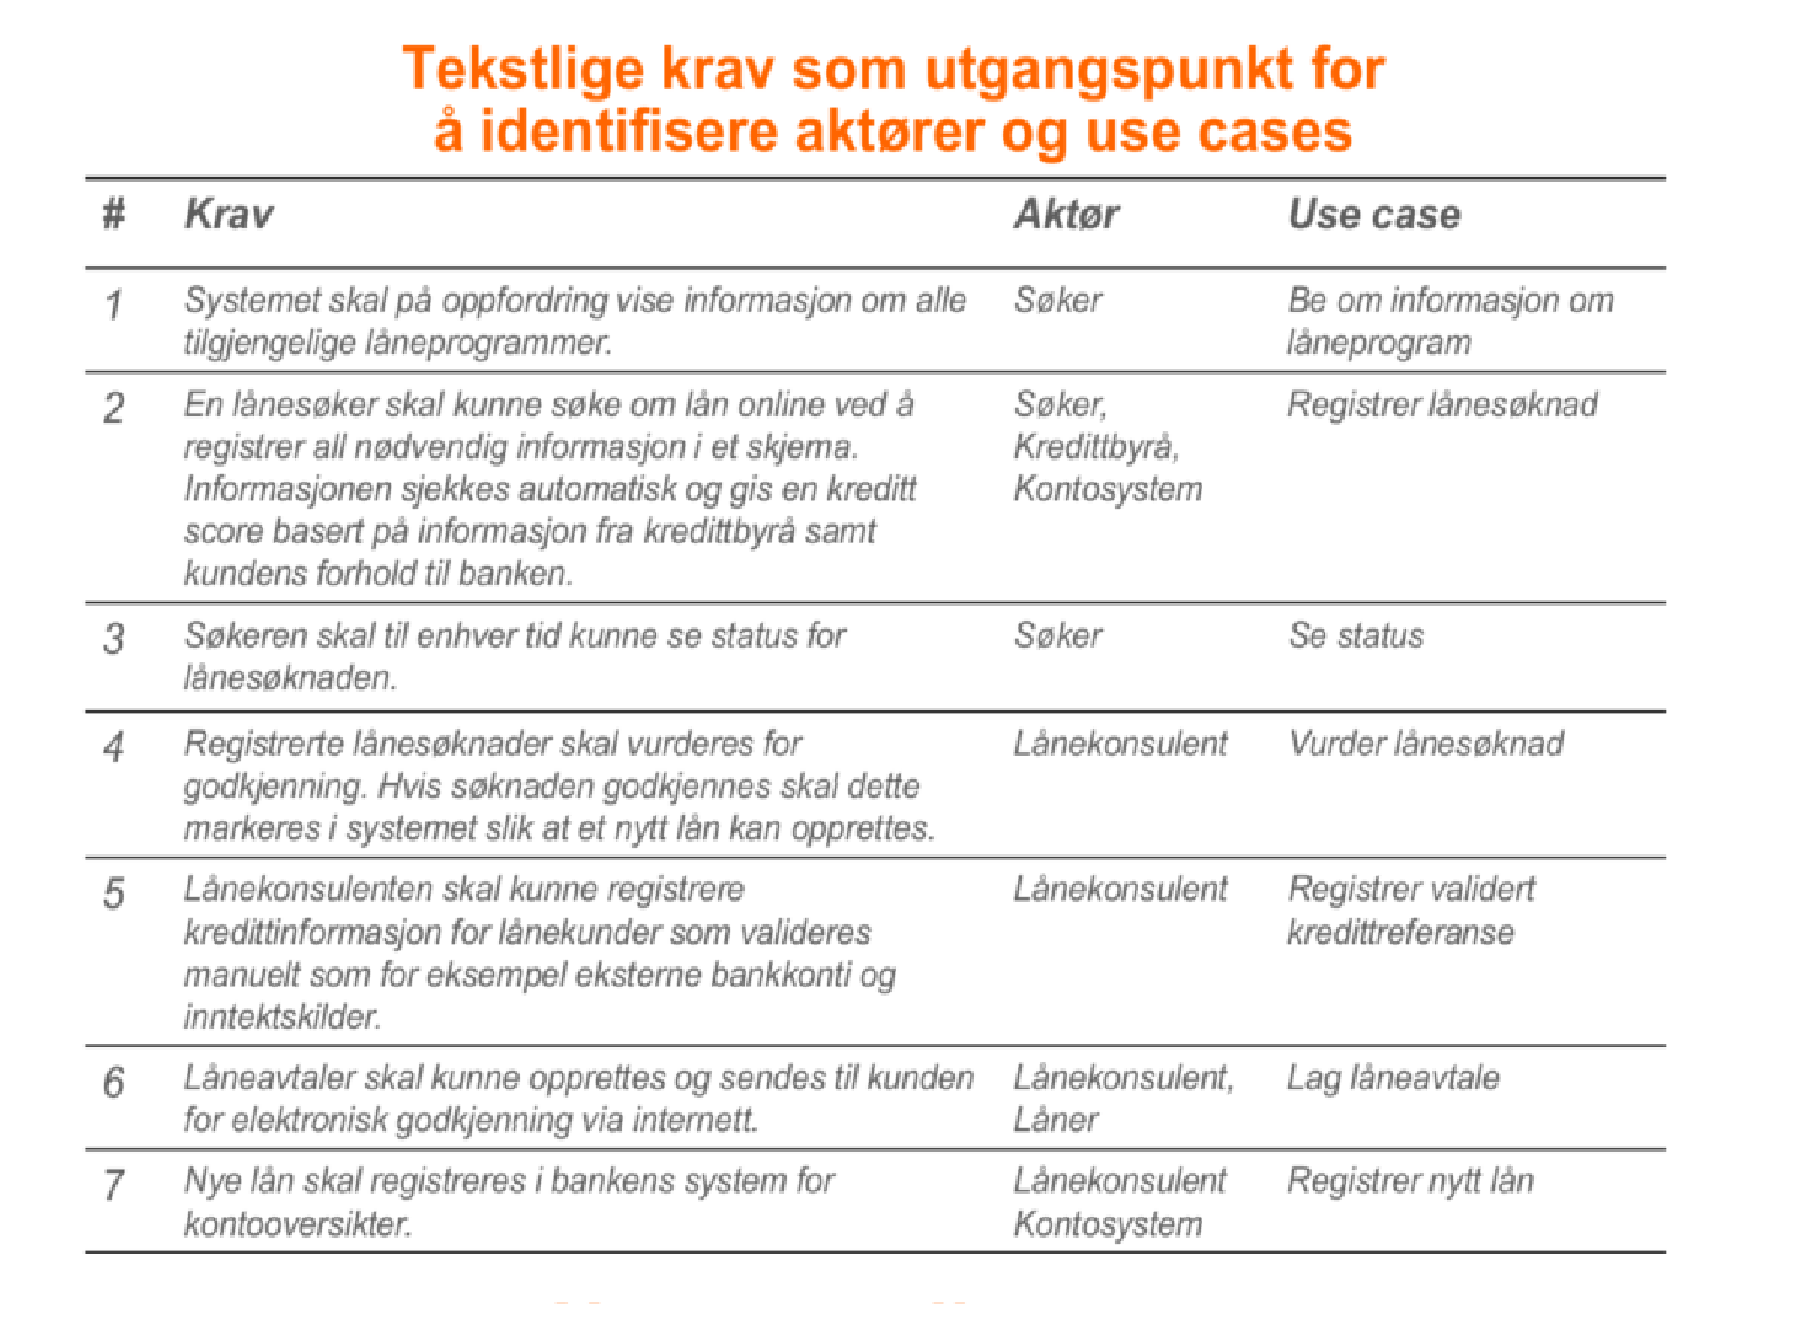
\includegraphics[width=0.7\textwidth]{./krav.eps}
    \caption{\label{fig:krav}Eksempel på kravtabell til et casediagram}
    \end{figure}
    \begin{figure}[htb]
    \centering
    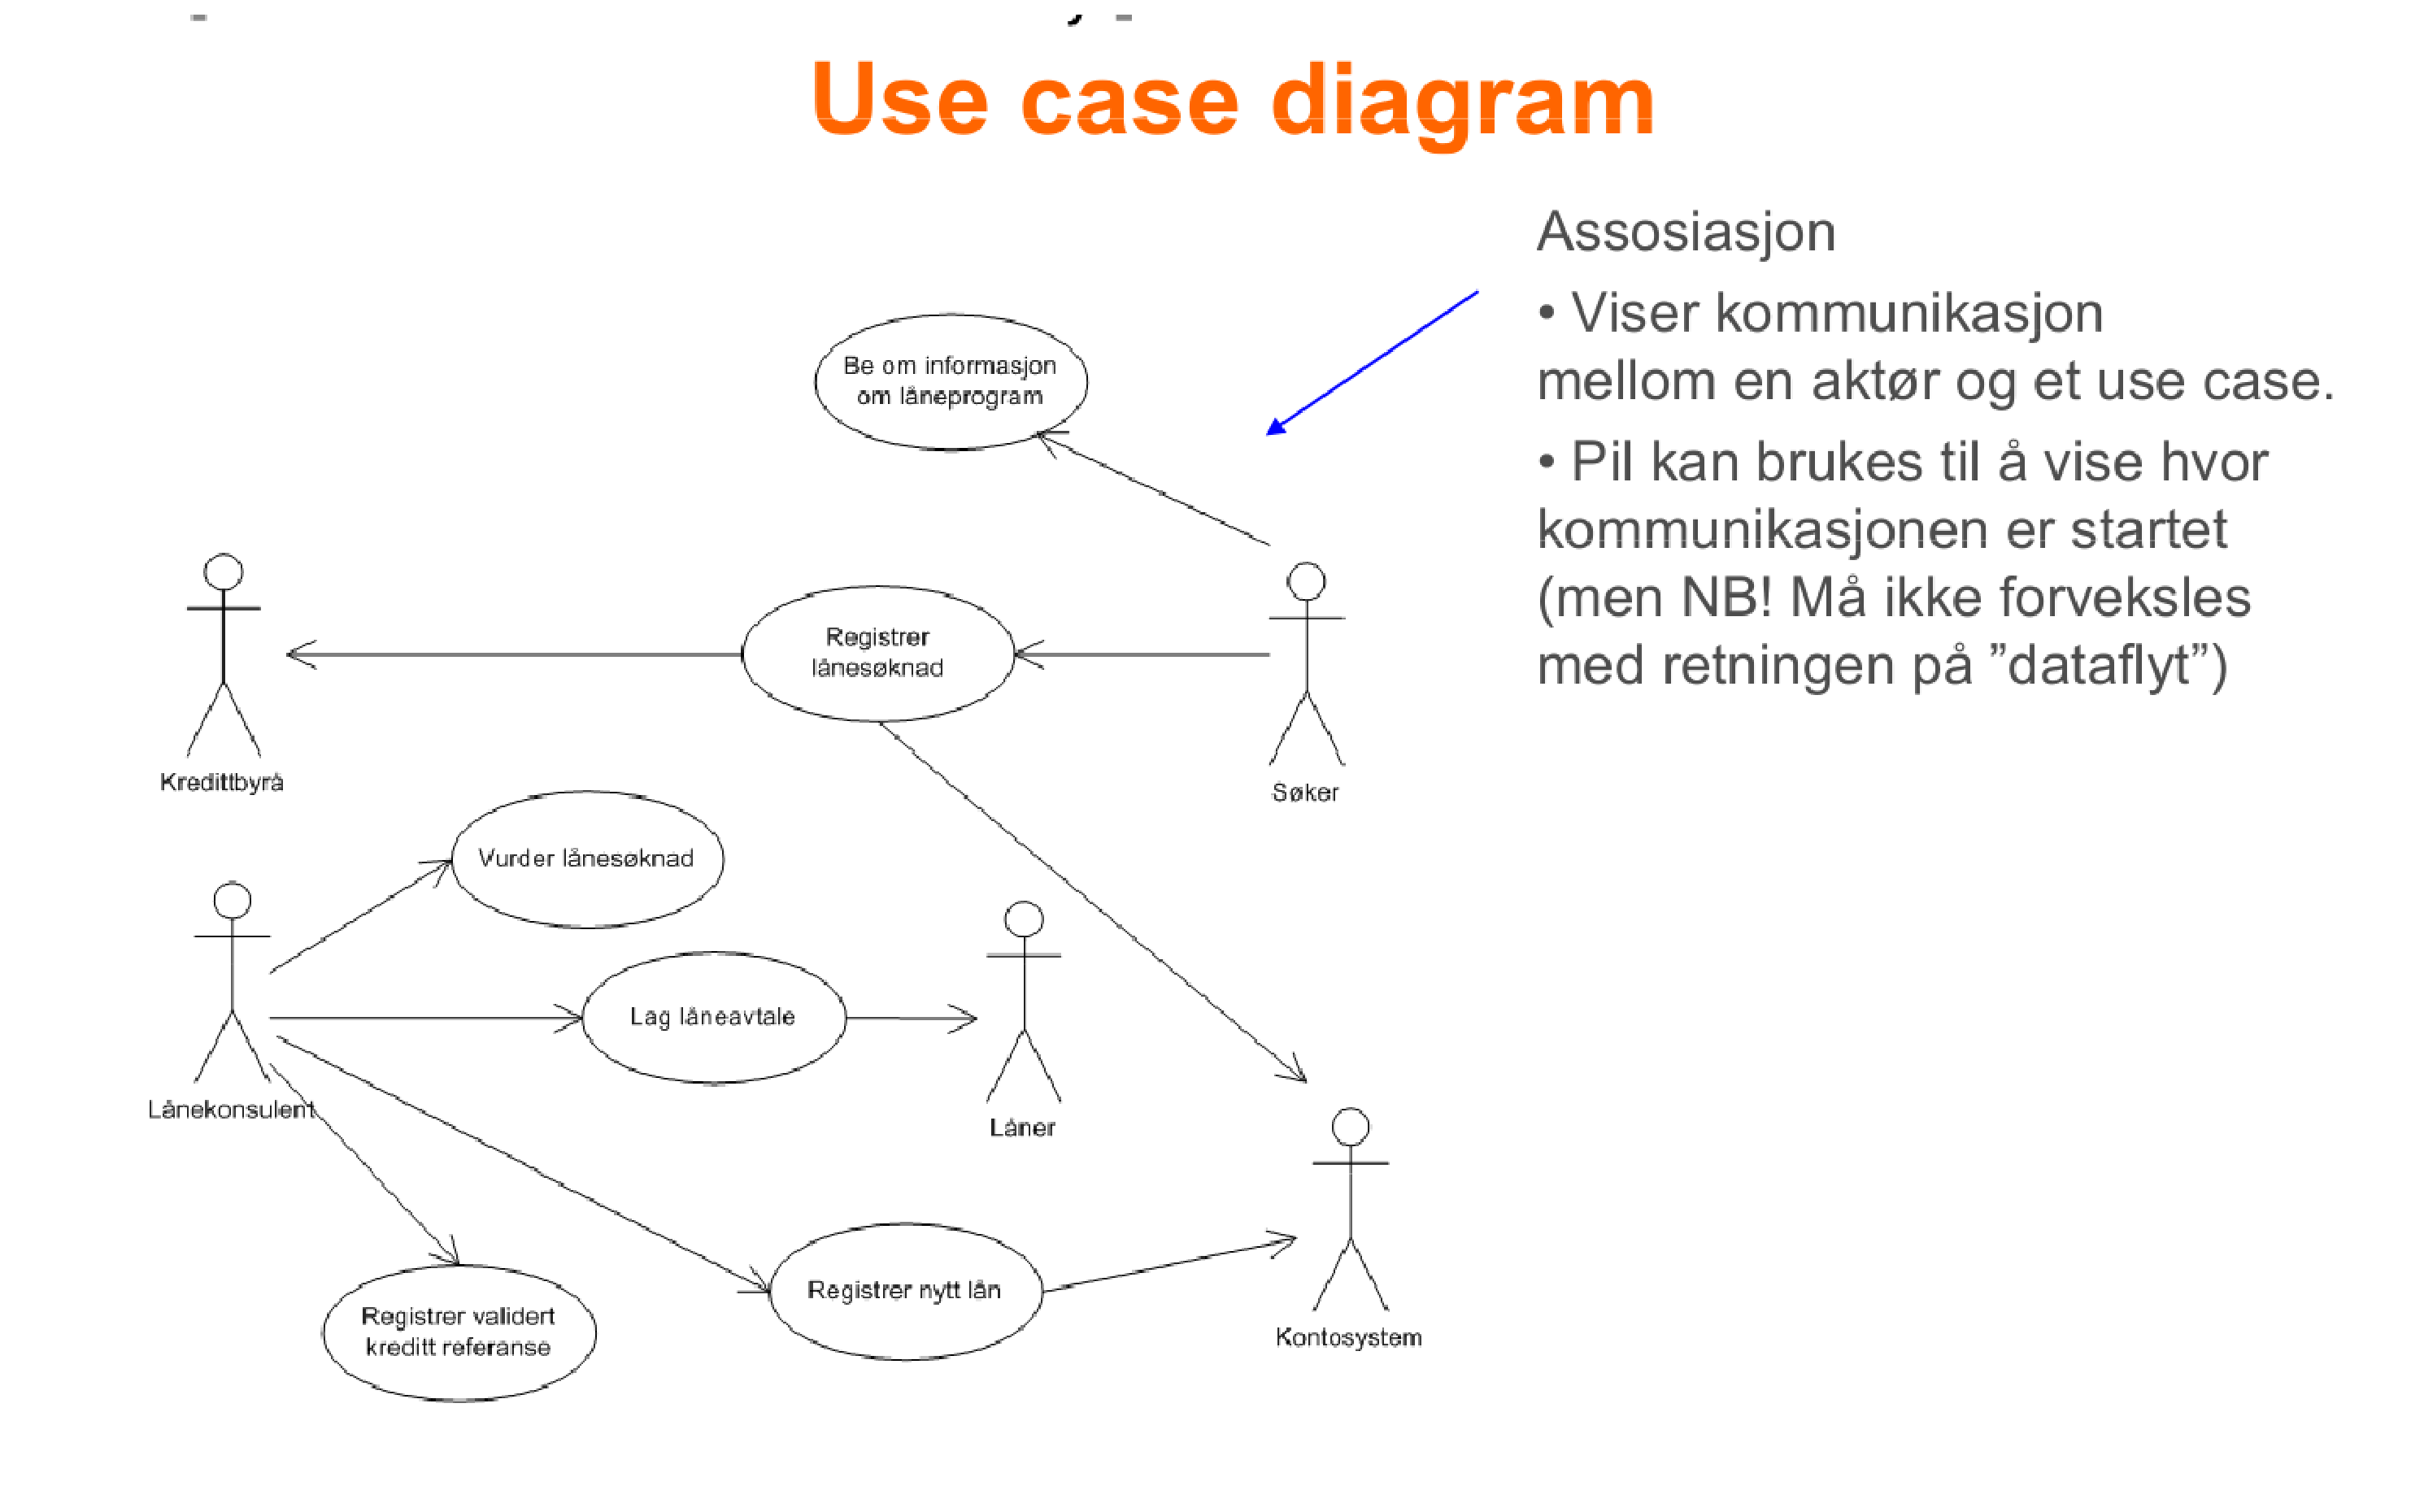
\includegraphics[width=\textwidth]{./case.eps}
    \caption{\label{fig:case}Eksempel på casediagram fre kravtabellen}
    \end{figure}
\begin{itemize}

\item \label{extend}extend\\
\label{sec-7.2.1.1}%
Utvider funksjonalitet, f.eks. i alteriantiv flyt.

\item \label{include}include\\
\label{sec-7.2.1.2}%
F.eks. hvis flere use case utfører samme prosedyre, kan vi lage use case av det, og include.


\item Hovedflyt\\
\label{sec-7.2.1.3}%
Brukes for å beskrive hvordan systemet skal fungere ut i fra Use case diagrammer
     og gjør det enklere å se hva som kan gå galt, og dermed gi alternative flyt

     eks. basert på use case diagrammet over

\begin{enumerate}
\item Søkeren fyller ut online lånesøknad
\item Søkeren sender søknaden til banken via internett
\item Systemet validerer informasjonen i lånesøknaden ved å 
        sjekke at den er så korrekt og komplett som mulig
\item Systemet innhenter kredittrapport for søkeren fra et
        eksternt kredittbyrå for kredittraport.
\item Systemet henter søkerens kontohistorie med banken
        fra kontosystemet
\item Systemet beregner søkerens kredittscore basert på
        kredittrapport og kontohistorie
\item Systemet informerer søkeren via e-mail om at søknaden 
        er mottatt og blir vurdert
\item Systemet setter status på lånesøknaden til ``Initiell
        kredittsjekk ferdig
\item Systemet allokerer lånesøknaden til en lånekonsulent 
        for videre behandling
\end{enumerate}


\item Pre- og postbetingelser\\
\label{sec-7.2.1.4}%
Use case ``Vurder lånesøknad'':

     \textbf{Prebetingelse:}
\begin{itemize}
\item Lånesøknaden har status ``Initiell kredittsjekk ferdig''
\end{itemize}
     \textbf{Postbetingelse: (en av de)}
\begin{itemize}
\item Lånesøknaden har status ``Godkjent''
\item Lånesøknaden har status ``Informasjon mangler''
\item Lånesøknaden har status ``Avslått'' og søker har fått
       beskjed om at søknaden er avslått
\end{itemize}
    
\end{itemize} % ends low level
\subsection{Datamodeller}
\label{sec-7.3}


   Datamodeller er digrammer som beskriver systemet på en objektorientert-lignende måte, 
   bare med dataen i systemet, istedenfor objektene. Man tegner opp enheter, attributter, 
   tjenester og deres relasjoner (med navn og antall/forhold/relasjoner). 

   Herunder kommer CRC-kort som beskriver hva objektene må vite om seg selv, og hvilke andre
   objekter som den har relasjoner til, hvordan skal den få tak i informasjon, hva 
   slags objektdet er - kant, kontroll, eller foretningsobjekt
   
   \begin{figure}[htb]
   \centering
   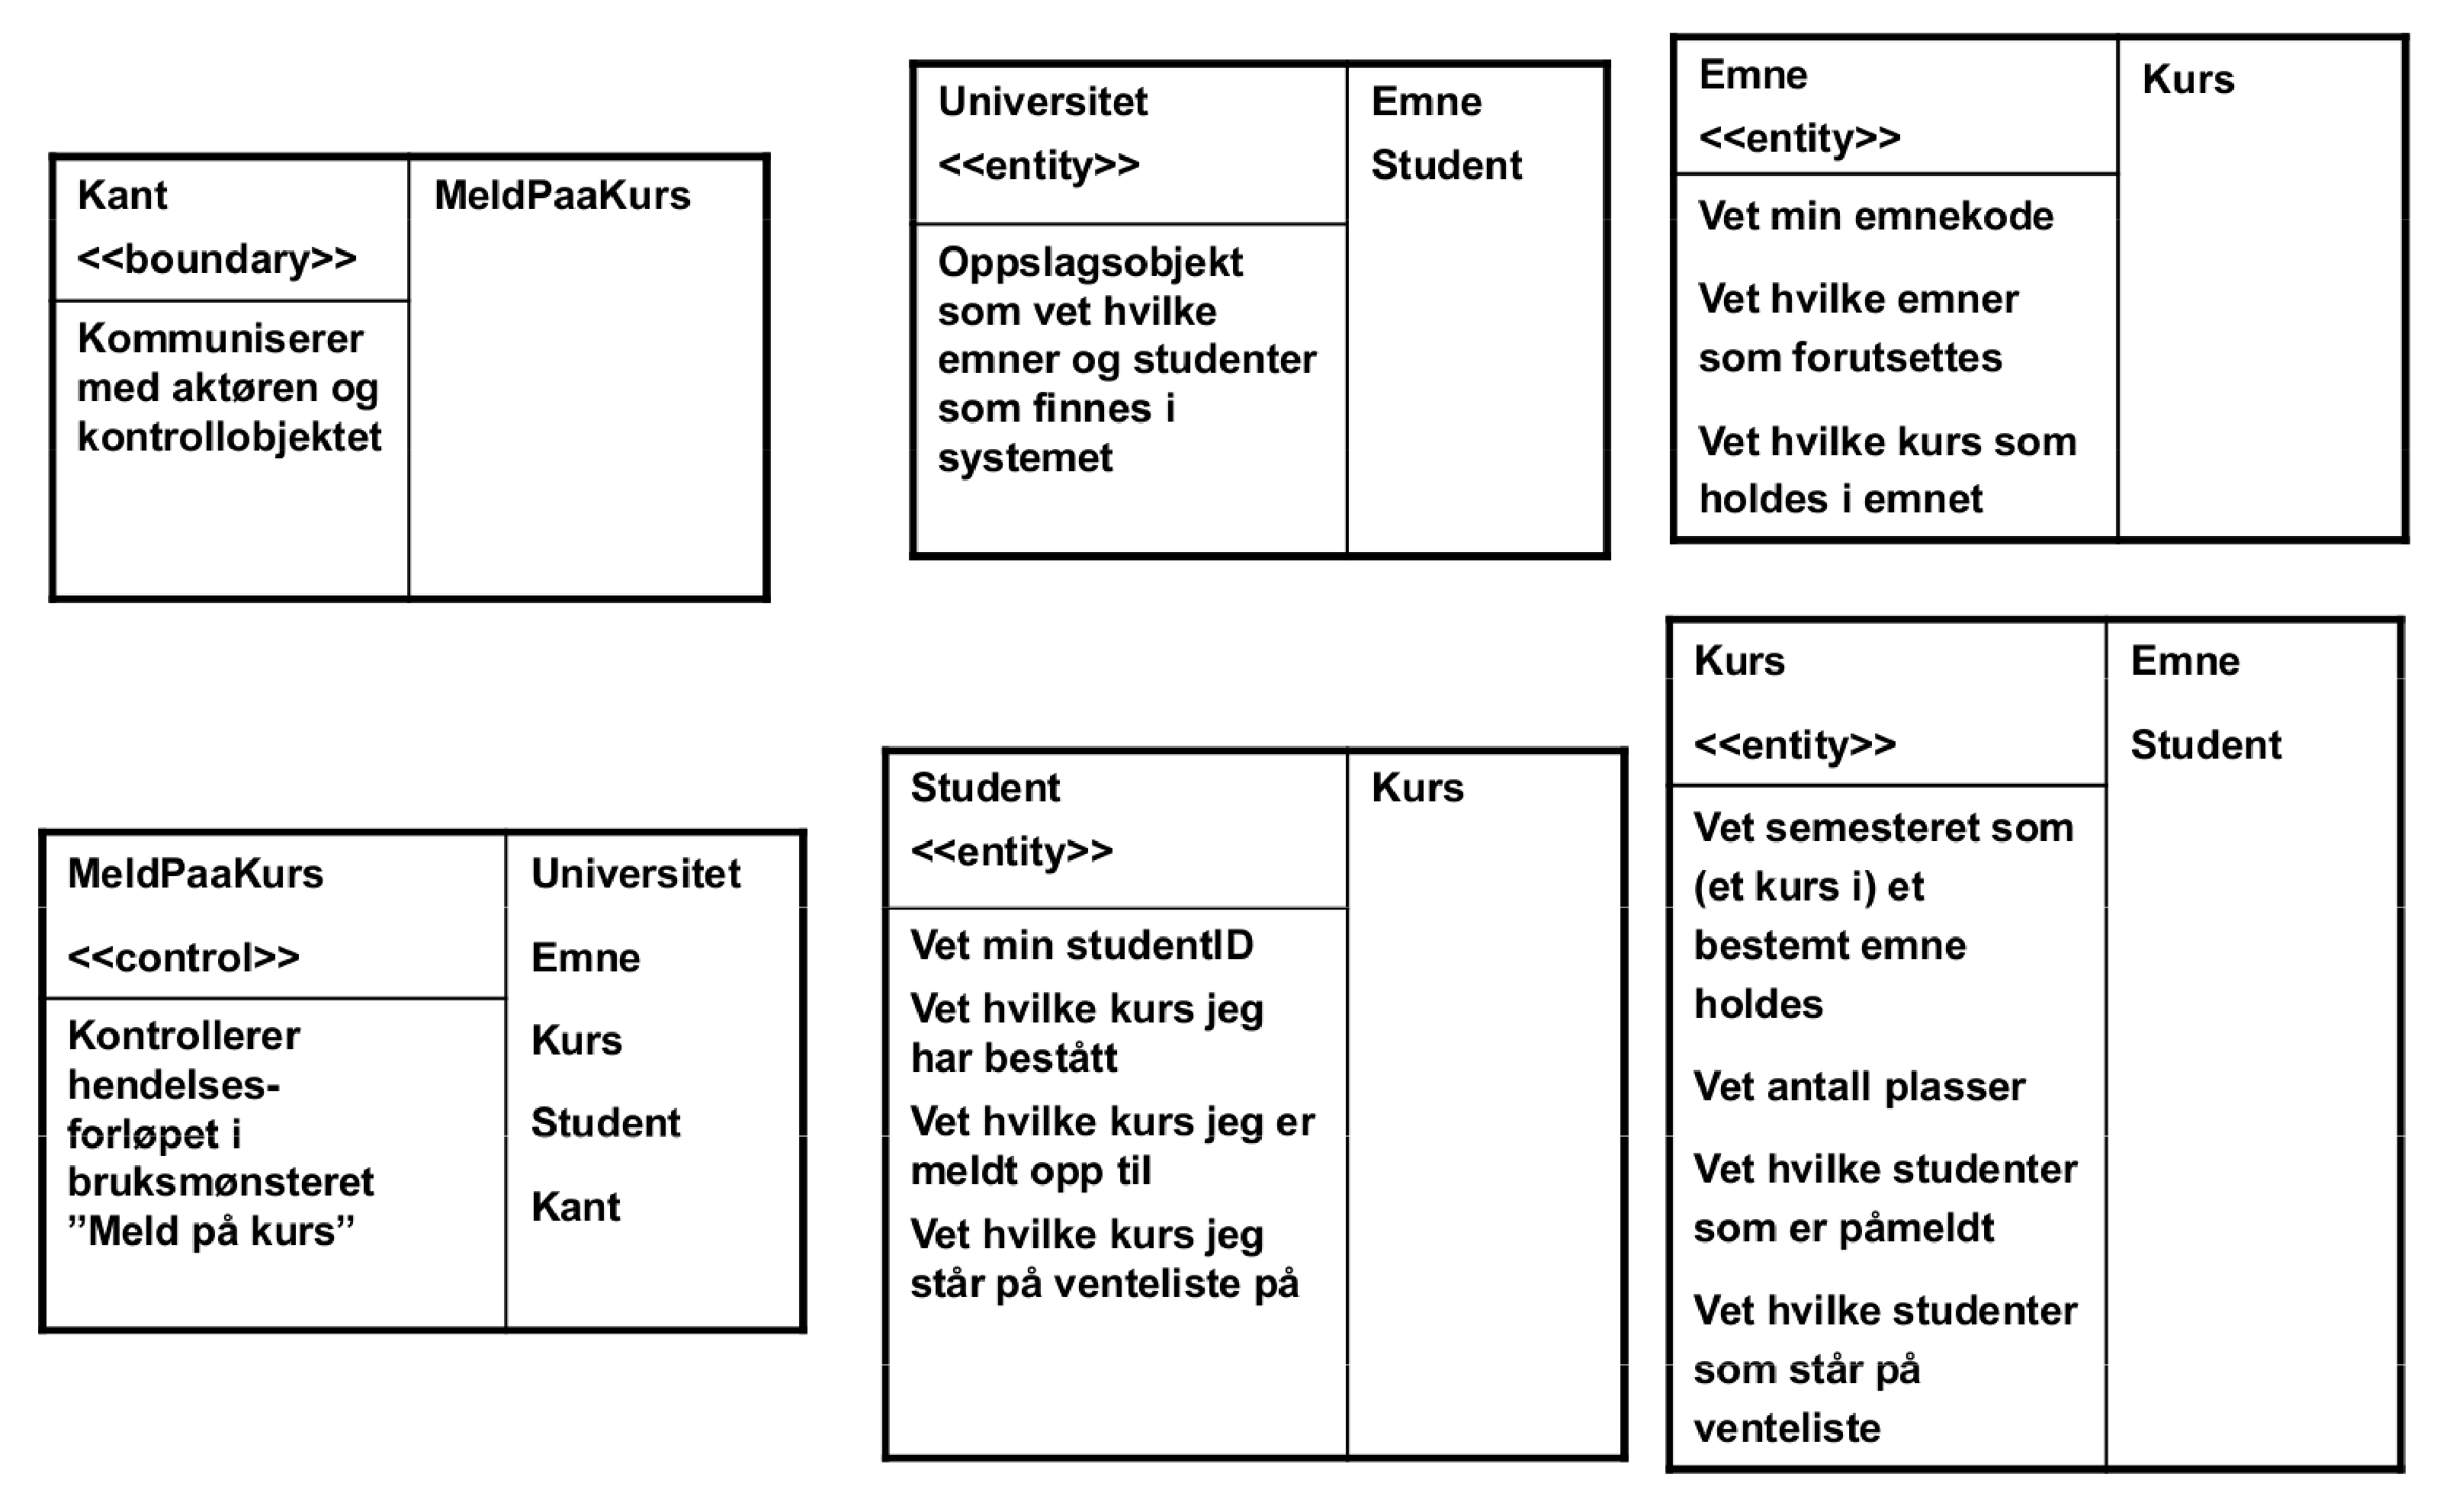
\includegraphics[width=\textwidth]{./CRC.eps}
   \caption{\label{fig:CRC-kort}Eksempel på CRC-kort}
   \end{figure}
\subsection{Objektmodeller}
\label{sec-7.4}


   Mye brukt i programvareutvikling, med objektorienterte språk. 
   Representerer systemet i en objektorientert måte, med UML. 
   Ofte er denne metoden veldig naturlig, siden den beskriver 
   virkeligheten på en naturlig måte, med objekter. 

   Objekter kan også arve egenskaper fra mer genrelle objekter i ett klassehierarki. 
   Spesialiserte objekter kan så legge til egne atributter og egenskaper.
\subsubsection{Domenemodeller}
\label{sec-7.4.1}

    Enkle klassediagrammer, uten metoder. Skal beskrive virkeligheten. Tegne opp relasjoner.

    Domenemodeller er nyttig i forbindelse med use case modellering fordi
\begin{enumerate}
\item Domenemodellen fanger opp informasjon om objekter i use casene og er
       et viktig verktøy for at use casene er beskrevet med riktig detaljeringsnivå
\item Klassene i domenemodellen kan brukes i utforming av mer presise pre- og postbetingelser
\end{enumerate}

    Hensikten med domenemodellen er å forstå objektene og få en oversikt over terminologi.
\begin{itemize}

\item Forretningsobjekter\\
\label{sec-7.4.1.1}%
De har evig liv. Lagrer i database.

\item Kontrollobjekter\\
\label{sec-7.4.1.2}%
Kontrolerer handlingsforløpet.

\item Kantobjekter\\
\label{sec-7.4.1.3}%
Kommniserer med brukere.

\end{itemize} % ends low level
\subsubsection{Sekvensdiagrammer}
\label{sec-7.4.2}

    Bygger på domenemodellen og objektene som er definert der
    og viser en interaksjon mellom aktører og objekter i systemet for
    et bestemt bruksmønster.
    
    Det er ofte nyttig med sekvensdiagrammer for å identifisere (og
    spesifisere bruken av) metodene til objektene i systemet

    \begin{figure}[htb]
    \centering
    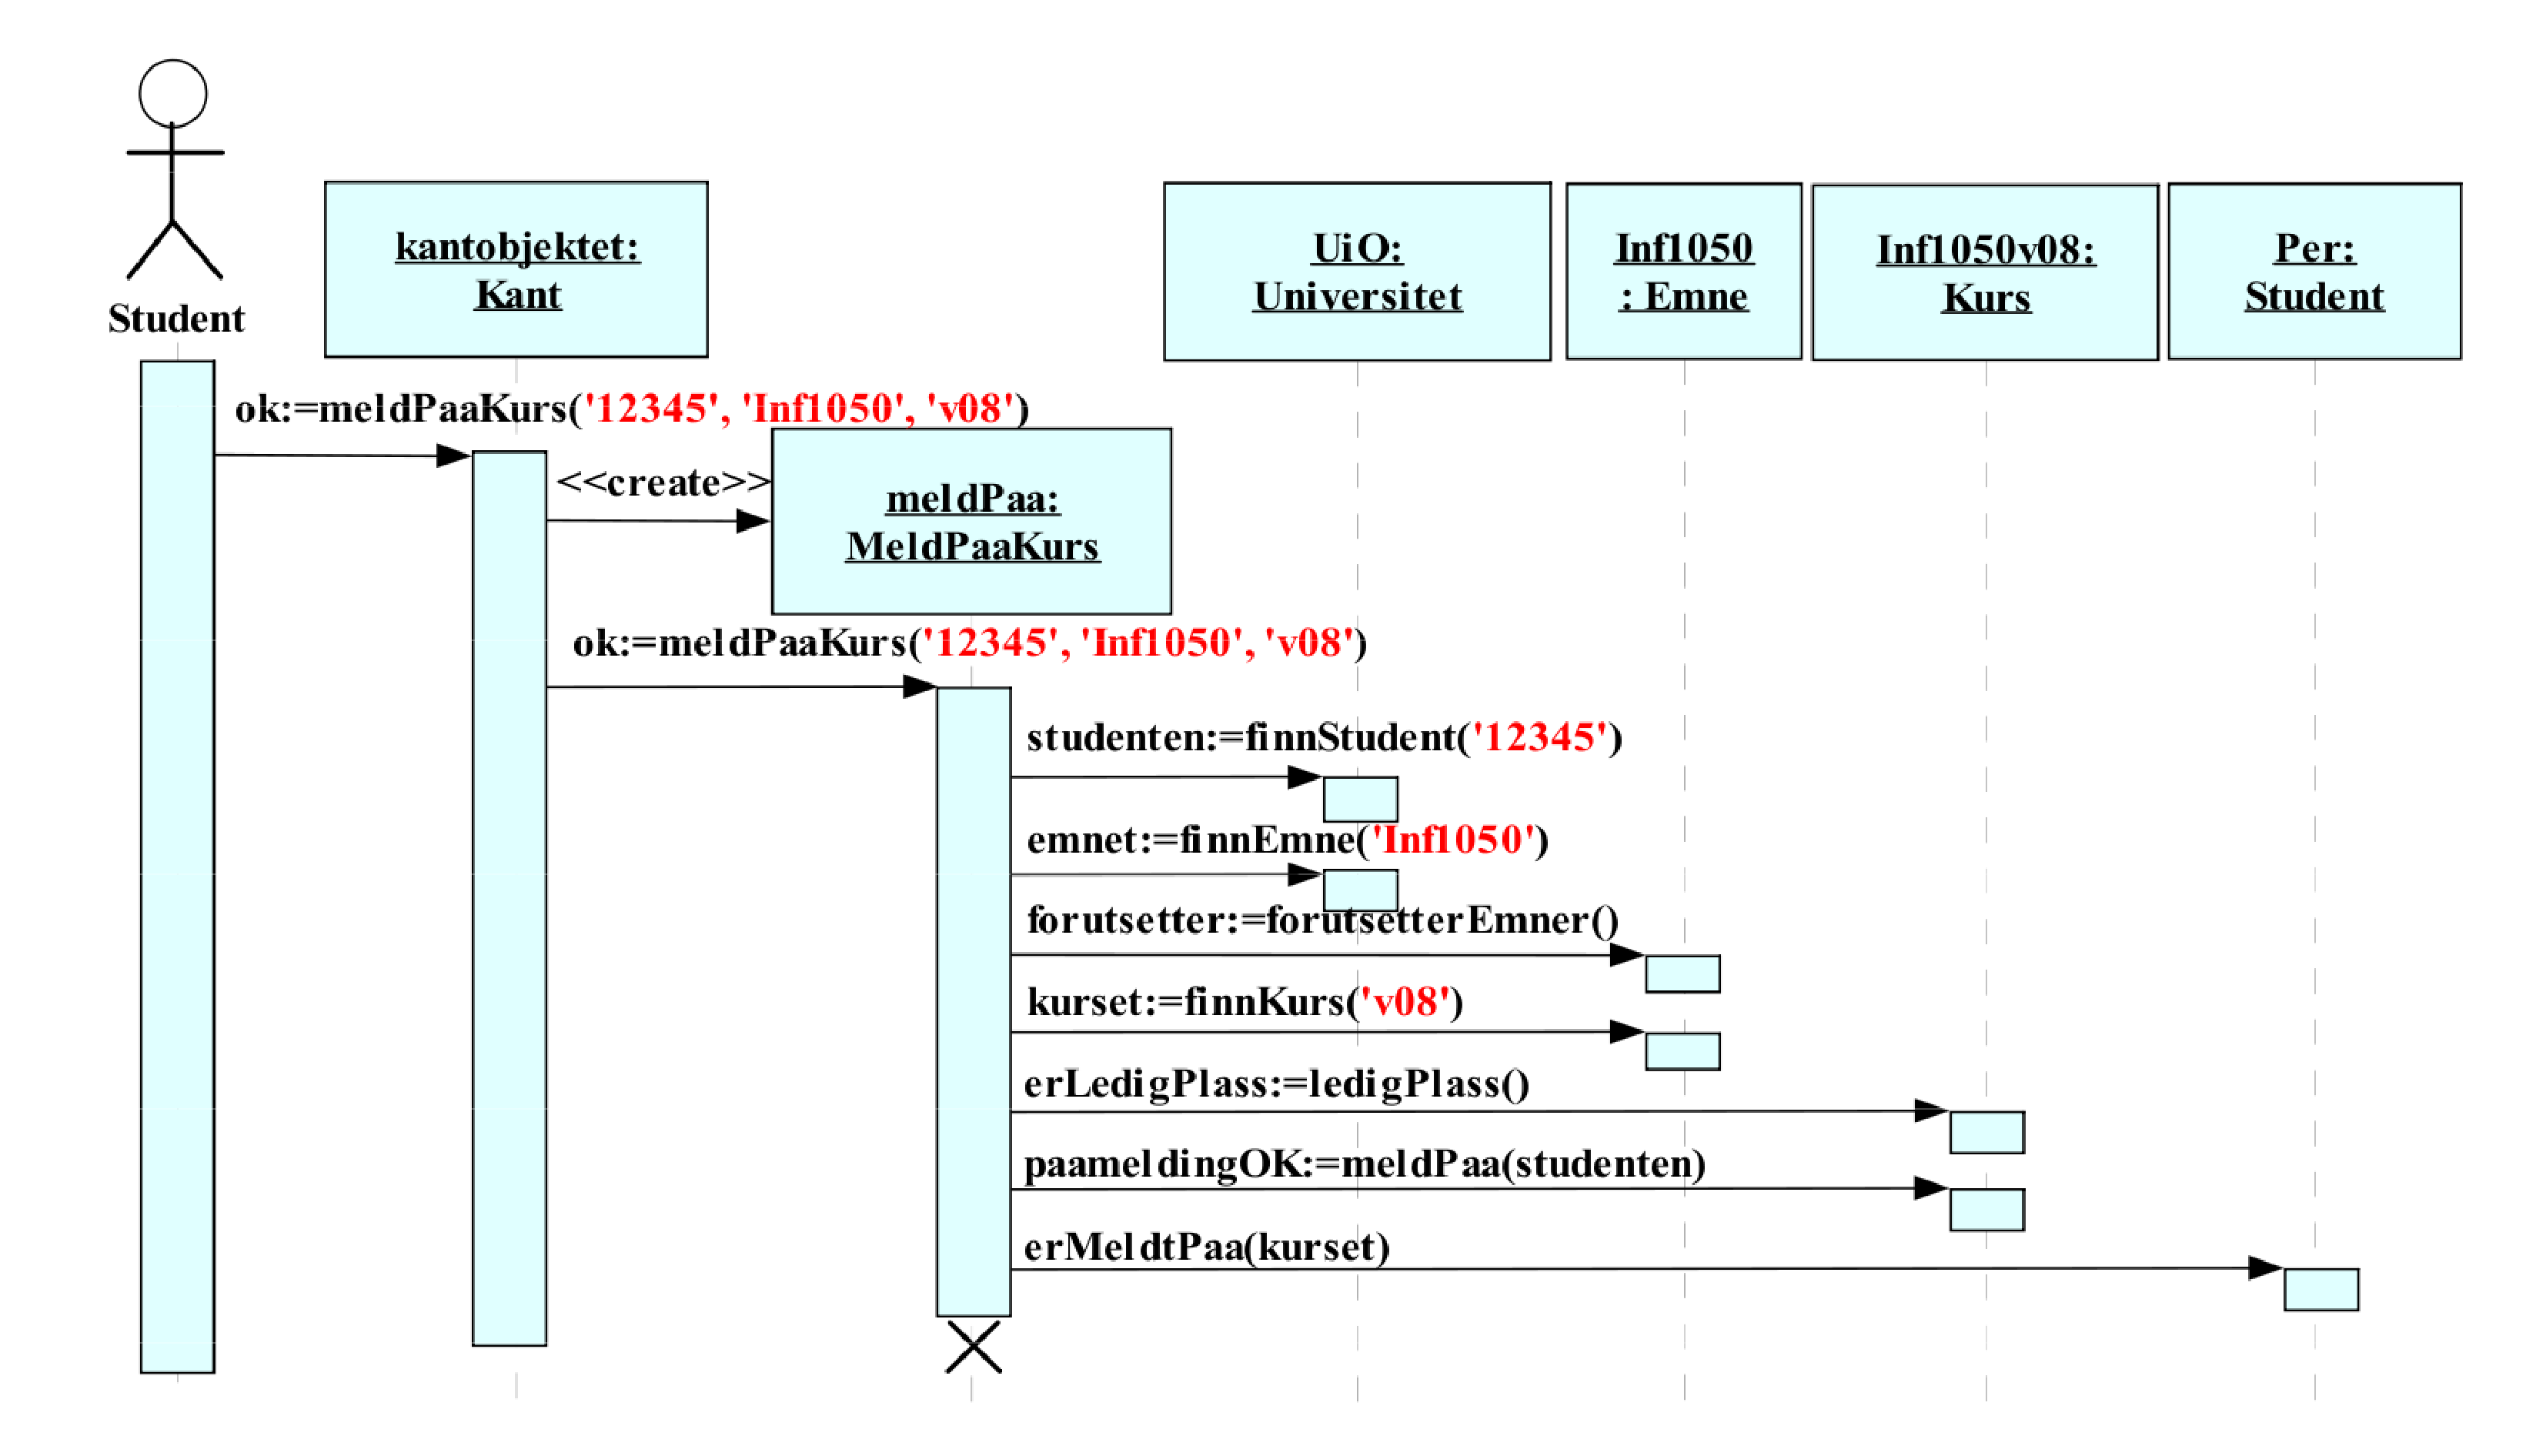
\includegraphics[width=\textwidth]{./sekvensdiagram.eps}
    \caption{\label{fig:sekvensdiagram}Eksempel på sekvensdiagram}
    \end{figure}
\subsection{Structured methods}
\label{sec-7.5}

   Karakteristikker:

\begin{itemize}
\item Brukes til kravspesifisering og systemdesign.
\item Dele prosjektet i veldefinerte aktiviteter.
\item Bruke diagrammodelering etc. på prosjektet.
\item Gi en god og strukturert definisjon av systemet.
\item Skal forstås av klient og utvikler.

    Ofte bruker man avanserte \textbf{CASE} (Computer-aided software engineering)-verktøy, 
    for å hjelpe til med denne prosessen. Det er verktøy som kan alt fra datamodelering, 
    automatisk generering av kildekode, og brukergrensesnitt-manipulering.
\end{itemize}
\subsection{Metode for ansvarsdrevet OO - INF1050-metoden}
\label{sec-7.6}

   Analyse av krav
\begin{itemize}
\item Identifiser krav
\item lag høynivå bruksmønsterdiagram
\item Spesifiser hvert bruksmønster tekstlig med hovedflyt og alternativ flyt
\end{itemize}

   Objektdesign, for hvert bruksmønser:
\begin{itemize}
\item Identifiser objekter, fordel ansvar (CRC)
\item Lag sekvensdiagram
\item Lag klassediagram
\item Lag klassediagram på systemnivå
\end{itemize}
\section{Kapittel 13 - Applikasjons-arkitektur}
\label{sec-8}
\subsection{Data-processing systems}
\label{sec-8.1}

   Får input-data fra database, eller filer, som den utfører en prosess på og sender det 
   ut igjen, enten tilbake i databasen, eller printe ut i ny fil.

   Slike prosesser er naturlig å representere i data-flyt-diagram-representasjoner. 
\subsection{Transaction-processing system}
\label{sec-8.2}

   Programmer som prosesserer spørringer mot databaser, eller oppdateringer av databaser. 
   Man sørger for at alle handlinger utføres trygt, før det speiles i databasen, slik at ikke databasen blir kurupt eller inkonsistent.
\subsection{Event-processing system}
\label{sec-8.3}

   Programmer som prosesserer hendelser i interfaces, gjort av brukeren, i en tilfeldig rekkefølge. 
   F.eks. Word Processors, bildebehandlingsprogrammer og spill.

   En del av disse, f.eks. teksteditorer har behov for svært rask behandling av data, 
   etter spesifikke eventer, og endringen foregår direkte i en buffer i minnet.
\subsection{Language-processing system}
\label{sec-8.4}

   Tar et naturlig, eller artificial konstruert språk, og generer en annen form 
   for representasjon som output. Vanligste eksemplet er \textbf{compilers}. Denne komponenten kan 
   være hardware (de fleste kompilatorer) eller software (slik Java er). 
\section{Kapittel 23 - Software-testing}
\label{sec-9}
\subsection{Kvaliteter vi trenger i produktene:}
\label{sec-9.1}

\begin{itemize}
\item Korrekt programvare
\item Pålitelighet
\item Robust
\item Ytelse
\item Brukervennlig
\end{itemize}

   Vi kan lete etter feil allerede i dokumentasjonen.
  
   Continuity properties gjelder ikke for software engineering, slik det gjør for andre ingeniørdisipliner.

\begin{itemize}
\item Komponent-testing: 
     Teste deler av systemet.
\item System-testing: 
     Teste hele systemet. Tester også funksjonelle og ikke-funksjonelle krav.
\end{itemize}

   Tester av to grunner: 
\begin{itemize}
\item For å demonstrere for kunde og utvikler at det fungerer tilfredsstillende.
\item For å avsløre feil eller mangler i programvaren.
\item Skrive tester for å sjekke krav. Trenger ofte flere tester for å få det til.
     Testing kan kun avsløre feil, ikke fraværet av feil.
\end{itemize}

   Problemer oppstår ofte når man kombinerer funksjoner i programmet.
   Vanlig prosedyre er at utviklere tester sine egne komponenter og sender de videre til teamet som integrerer dem, og tester hele systemet.
\subsection{System-testing}
\label{sec-9.2}


   Å teste integreringen av to eller flere komponeneter, og at alt går som det skal.
   Man tester for hvert komponent-inkrement, for å teste alle kombinasjoner.
\subsubsection{Release-testing:}
\label{sec-9.2.1}

    Sender beta-utgaver til folk, for å kontrollere at den tilfredsstiller kravene og at den ikke feiler ved vanlig bruk.

    Man prøver altids input som har størst sannsynlighet for å gi en feil i programmet. (Test alle error-meldinger, test buffer overflow, repeter samme input flere ganger, tving frem feil output, tving frem for store eller for små outputs).
\subsubsection{Performence-testing:}
\label{sec-9.2.2}

    Tester om hastighet/påletelighet/stabilitet er som det skal være. 
    Stresstester systemet utenfor for kravene som er definert i kravene, 
    og sjekker om den feiler ``soft'' eller skaper store problemer. 
\subsubsection{Komponent-testing}
\label{sec-9.2.3}


    Å teste enkeltkomponeneter. Hovedsaklig utvikler som gjør den jobben. 
    Enten indivudelle metoder eller funksjoner i ett objekt, eller objekt-klasser 
    med flere attributter og tilhørende metoder.
\subsubsection{Interface-testing:}
\label{sec-9.2.4}

    Teser interface-komunikasjon mellom flere komponenter.
    Test Case-design

    Designer tester. Input og predikert output. Skal være effektive til å teste systemet, og finne eventuelle feil og at systemet tilfredsstiller kravene.
\subsubsection{Kravbasert testing:}
\label{sec-9.2.5}

    tester kravspesifikasjonene, om de er møtt. Gjøres i system-testing-delen.
\subsubsection{Structural testing:}
\label{sec-9.2.6}

    Passer på at alle delene av kodene kjøres minst en gang.
\subsubsection{Partition testing:}
\label{sec-9.2.7}

    Kan teste med kun en input av input med like karakteristikk. F.eks. ett positiv tall, 
    ett negativt etc. Prøver ofte med atypiske verdier, siden utviklere ofte glemmer dette. 
    ved inputverdier velger du verdier midt i områdene og verdier på begge sider av verdigrensene.
\subsubsection{Structural testing(white-box):}
\label{sec-9.2.8}
\subsubsection{Path testing:}
\label{sec-9.2.9}

    Vi tegner opp ett diagram over alle mulige grenveier det er mulig å kjøre igjennom. 
    Alle løkker og if-else-settninger blir grener  og looper i programmet. Så sørger vi for 
    å gjøre testinger så hver kodeblokk blir kjørt minst en gang, og får testet alt med både true og false.
    
\subsection{Test-automatisering}
\label{sec-9.3}


   Testing er dyrt. Kom derfor raskt en del programvare som kan automatisere prosessen. 
   Kan holde orden på testdata, generere testdata, Oracle som predikerer forvenet resultat, 
   File comperator som sammenligner tester, Dynamic analyser som sjekker hvor ofte de firskjellige
   statementene blir kjørt. Og simulering i forskjellige varianter. F.eks. bruker-interaksjon.

   Testingsfasen er ofte estimert til å være 50\% av utviklingskostnadene.
\section{Kapittel 26 - Software cost estimation}
\label{sec-10}
\subsection{Software productivity}
\label{sec-10.1}

   Handler om å kartlegge produktiviteten til utviklerene, effektivitetskostnadene 
   for jobben, og fordele arbeidet utover. Har ofte behov for dette, for å senere 
   kunne gi en prisestimering. Kan ofte bruke antall linjer kode estimert, som en basis 
   for videre estimat. Eller hvor lang tid man bruker per funksjon i systemet. 

   LOC/pm er en måte å måle produktivitet på. LinsOfCode / programmer-months. 
   Denne effektiviteten avhenger av hvilket språk som brukes, da forskjellige språk, 
   krever forskjellig antall linjer kode, for å utføre samme prosedyre.

   Man kan også funksjons-punkt-estimering. Denne metoden kan gjøres på et tidligere 
   stadie en LOC, siden man vet det meste man trenger etter kravspesifisering etc.
\subsection{Estimation techniques}
\label{sec-10.2}

   Det finnes flere teknikker for å estimere prisen:

\begin{itemize}
\item Estimering basert på kostander til lignende prosjekter.
\item Leie inn flere eksperter, for så å sammenligne og diskutere deres estimeringer.
\item Parkison's Law: Sier at arbeid vil fylle ut tid som er satt til side.
\item Det kan avhenge av hva kunden er tilgjengelig av budsjett.
\end{itemize}

   Det er ofte lurt å bruke flere estimeringsmetoder, 
   for så å sammenligne dem til slutt. Varierer estimeringene kraftig, 
   kan man regne med at man ikke har nok informasjon.
\subsection{Algoritmic cost modeling}
\label{sec-10.3}

   Algorthmic cost modeling bruker en matematisk formel til å beregne tid og pris-estimatet, 
   som er regnet ut fra tidligere, fullførte prosjekter. En vanlig formel kan se slik ut 
   
   $Effort = A \times Size^B \times M$. 

\begin{itemize}
\item \textbf{A} er en faktor, som avhenger av organisasjonen sin praktisering og type programvare som skal utvikles.
\item \textbf{Size} er LOC eller funksjons-estimering, representert i funksjon eller object points.
\item \textbf{B} ligger mellom 1 og 1.5.
\item \textbf{M} er en multiplikator, avhengig av ting rundt utviklingsprosessen og erfaring til utviklere etc.
\end{itemize}

   I starten av estimeringsfasen vil nøyaktigheten variere fra 0.25X til 4X. Utover i prosessen 
   vil det bli tydeligere og tydeligere hvor lang tid det vil ta.. Det er viktig å derfor legge til rette, for å kunne endre rundt dette.

   \textbf{COCOMO} er en avansert standard for prisestimering, som har tre forskjellige detaljnivåer,
   og bruker en rekke forskjellige input til å estimere kostnader og tid, med varierende treffsikkerhet. 
\subsection{Product duration and staffing}
\label{sec-10.4}

   Programvare forventes å komme på markedet raskere og raskere, for å kunne konkurere med motstanderne. 
   Forholdet mellom utviklere og tid er ikke lineært, på grunn av kommunikasjon og management.

   COCOMO-modellen har en modell for estimere kalendertid (TDEV), 
   
   $TDEV = 3 \times (PM)^{(0.33+0.2 \times (B-1.01))}$.
   
\begin{itemize}
\item PM er innsats-estimering.
\item B er utregnet eksponent for COCOMO-modellen.

     Ofte trenger man heller ikke mange arbeidere i startfasen, men heller flere etterhvert. 
     Det er da viktig å ikke ta inn for mange arbeidere av gangen, da dette fører til problemer
     og kan senke prosessen. Det bør gjøres gradvis.
\end{itemize}
\section{PS2000}
\label{sec-11}

  Utviklet av Dataforeningen
\subsection{Bruksområde:}
\label{sec-11.1}

\begin{enumerate}
\item Drift av IT- løsninger

\begin{itemize}
\item Utstyr
\item Programmer
\end{itemize}

\item Livsløpsperspektiv

\begin{itemize}
\item Etablering
\item Ordinær drift
\item Avslutning
\end{itemize}

\end{enumerate}

   Eies av kunden og/eller leverandøren
   -Hvor det ikke er mulig eller hensiktsmessig å etablere nøyaktige eller detaljerte kontrakter.

   En IT-leveranser er for Maskinvare, programvare og tjenester.
   Formålet med kontrakt er konfliktforebygging og gjensidig forpliktelser.
   Mest viktig å fordele risiko?

   Har både interne og eksterne rammebetingelser man må ta hensyn til.
\subsection{prisformer}
\label{sec-11.2}

   PS2000 regulerer iterative eller smidige (agile) prosesser. 
   Kan benyttes både av private og offentlige aktører. Utviklet så begge parter tas vare på.

\begin{itemize}
\item Kontrakten er i større grad ett styringsverktøy. Basert på iterative metoder.
\item Regulerte forpliktelser i begge parter.
\item Håndtering av usikkerhet tilrettelagt.
\end{itemize}

  Ukentlig oppdatering av risikomatrise.

  Jo lengre ut i prosjektet man er, jo dyrere er endringer, 
  men desto mer vet man hva man ønsker av produktet, 
  og desto større nytte-effekt av endring. Dilemma!

  Fleksibel og oversiktelig.
\subsubsection{Fastpris}
\label{sec-11.2.1}

    knyttet til avtalt omfang.
\begin{itemize}
\item Kundeperspektiv

\begin{itemize}
\item Forutsigbart, men risikerer å få et avkortet produkt dersom
        leverandøren ikke vil jobbe utover fastpriskostnadene.
\end{itemize}

\item Leverandørperspektiv

\begin{itemize}
\item Også forutsigbart, men risikerer å jobbe gratis etter at 
        fastpriskostnadene er brukt
\end{itemize}

\end{itemize}
\subsubsection{Løpende timer}
\label{sec-11.2.2}

    fakurerer timer og annet.  
\begin{itemize}
\item Kundeperspektiv:

\begin{itemize}
\item Lite forutsigbart og risiko for store budsjettoverskridelser.
        vil dog kunne få levert et fullstendig produkt.
\end{itemize}

\item Leverandørperspektiv:

\begin{itemize}
\item Også lite forutsigbart, men får dekket faktiske utgifter
\end{itemize}

\end{itemize}
\subsubsection{Målpris}
\label{sec-11.2.3}

    basert på estimater og risikovrderinger. Justeres med incentiver og
    saksjoner.
\begin{itemize}
\item Kundeperspektiv og leverandørperspektiv

\begin{itemize}
\item Forutsigbart og eksplisitt håndtering av risiko og
        ansvarsfordeling. Rom for erfaringsbaserte vurderinger. Støtter samarbeid mellom kunde og
        leverandør. Krever ekstraarbeid for å vurdere risiko og usikkerhet. Krever at begge parter
        forstår incentiv-modeller.
\end{itemize}

\item Bruksområder

\begin{itemize}
\item Systemutvikling basert på relativt godt spesifisert behovsanalyse
\item Godt nok grunnlag for realistiske estimater
\item Erkjennelse av at krav og prioriteringer kan endre seg underveis
\end{itemize}

\item Fordeler og ulemper

\begin{itemize}
\item Relativ forutsigbar mht. kostnader
\item Klare leveranseavtaler mht. omfang og kalendertid
\item Rom for erfaringsbaserte justeringer i iterasjoner
\item Støtter integrert samarbeidsmodell
\item Felles incentiver om å levere kvalitet til avtalt tid og kostnad
\end{itemize}

\end{itemize}
\subsection{PS2000 vs andre kontrakter}
\label{sec-11.3}


   Kontraktsstandarden skiller seg vesentlig fra andre standarder i markedet. 
   Spesielt kan følgende trekkes frem: 

\begin{itemize}
\item Kontraktsstandarden er utviklet av kunder og leverandører i samarbeid, 
     slik at begge parters interesser er ivaretatt og balansert.
\item Kontraktsstandarden tilrettelegger for å fange opp den læring som foregår under gjennomføring av prosjektet. 
     Gjennomføringsmodellen består av 4 faser

\begin{itemize}
\item behovsfasen
\item løsningsbeskrivelsesfasen
\item en trinnvis konstruksjonsfase
\item godkjennings- og avslutningsfasen
\end{itemize}

\item Det er tilrettelagt for utstrakt bruk av motiverende økonomiske modeller i form av incentivordninger
     for at eventuelle tids- og kostnadsbesparelser kommer begge parter til gode og vice versa. 
     Det skal utarbeides en usikkerhetsanalyse som legges til grunn ved valg av spesifikke incentiver.
\item Samhandling mellom kunde og leverandør forbedres 
     ved at kontraktsstandarden legger opp til et integrert samarbeid 
     og en effektiv og separat prosess for eventuell konfliktløsning.
\item Kontraktsstrukturen med forhåndsutfylte bilag og veiledning gjør det enklere å utforme spesifikke kontrakter tilpasset ulike behov. 
     Alle referanser i de generelle kontraktsbestemmelsene er utdypet i bilagene.
\end{itemize}
\subsubsection{Andre kontrakter}
\label{sec-11.3.1}

    
    Begge de to andre avtalene som er pressentert på forelesninger er basert
    på å ivareta en interessent sin interesse, og ikke begge, PS2000 er unik der
    og det er derfor vi nesten utelukkende har om PS2000
\begin{itemize}

\item IKT Norge:\\
\label{sec-11.3.1.1}%
Laget for å ivareta leverandørs interesser
\begin{itemize}

\item Standardavtale om systemutvikling\\
\label{sec-11.3.1.1.1}%
\item Standardavtale om systemutviklingsprosjekt\\
\label{sec-11.3.1.1.2}%
\end{itemize} % ends low level

\item Statens standardavtaler (DIFI):\\
\label{sec-11.3.1.2}%
Laget for å ivareta kunders interesser
\begin{itemize}

\item Programmutviklingsavtalen\\
\label{sec-11.3.1.2.1}%
\end{itemize} % ends low level
\end{itemize} % ends low level
\subsection{Oppbygging av PS2000}
\label{sec-11.4}

   Kontrakten er delt inn i

   Del1: Kontraktsdokument 
   Del2: Generelle kontraktsbestemmelser 
   Del3: Kontraktsbilag
\section{Kapittel 11 (Ikke hoved) - Arkitekturdesign}
\label{sec-12}

  Valg av arkitektur-rammeverket influerer viktige deler av systemet, som hastighet, sikkerhet og tilgjengelighet. 

  Store systemer deles inn i subsystemer. ARkitekturdesign er å fastsette disse subsystemene, og kommunikasjonen dem imelom.
  
  Skisse en grunnleggende struktur av systemet, og hovedkomponentenene og kommunikasjonen i mellom.

  Er mer en bestemmelseprosess enn en aktivitet. 

  Finnes to typer dataarkitekturer. Sentral database, eller lokal database, hvor subsystemene sender dataen til og fra hverandre. Fordelen med klient-server-modellen er at den er disitrbuert, og det er lett å oppgradere og fordele belasten.

  \textbf{Layered-modellen} organiserer systemet i lag. Kan endres, så lenge interfacet er det samme. Negative siden er at flere lag kan gjøre at systemet går tregere.

  Et subsystem skal være uavhengig, og fungere uavhengig av de andre subsystemene. Mens en modul er en litt mindre enhet, som ofte benytter seg av tjenester i andre moduler etc.

  Finnes to måter å visualisere systemarkitekturen på.

\begin{enumerate}
\item Objektorientert
     der hvert objekt er ett subsystem. En fordel med dette er at objektene kan gjenbrukes.
\item Funksjons-orienter 
     der man har input-data som går gjennom forskjellige funksjoner (subsystemer) og får til slutt en output.
\end{enumerate}
\section{Kapittel 12 (Ikke hoved) - Distributed system architecture}
\label{sec-13}

  Så og si alle større systemer i dag, er distrubert over flere maskiner. Det har en del fordeler, blant annet

\begin{itemize}
\item Deling av resursser, både hardware og software.
\item Ofte designet rundt åpne standarder og protokoller.
\item Skalerer lett.
\item Stor feiltolleranse, annen server kan raskt slå inn i steden hvis man har flere.
\end{itemize}

  Ulempene er

\begin{itemize}
\item Kompleksitet.
\item Sikkerhet pga traffiken må gå over nettverk, mulighet for eavsdropping.
\item Kan være vanselig å drifte store distribuerte systemer.
\end{itemize}

  Generelt sett kan vi si at vi har to typer distribuerte systemer.

\begin{itemize}
\item \textbf{Klient-server}. Tilbyr tjenester, som klientene spør etter.
\item \textbf{Distribuert objekt-arkitektur}. For objektene er forespørsler 
    fra klient og andre objekter akkurat det samme.
\end{itemize}

  Multiprosessor-arkitektur, lar flere prosesser i samme system, kjøre på forskjellige prosessorer.

  Klient-server-arkitetur kan ha to former.

\begin{enumerate}
\item Tynn-klient.

\begin{itemize}
\item klienten vil bare mota og sende informasjon, bare ansvarlig for å presentere informasjonen
\item Serveren gjør all prossessering og datamanagement
\end{itemize}

\item Tykk-klient.

\begin{itemize}
\item Klienten har applikasjonslogikk i tillegg til brukerinteraksjon
\item Serveren har bare ansvar for datamanagement (serveren brukes som database)
\end{itemize}

\end{enumerate}

  Mobile klienter er ofte en liten mellomting av disse.

  CORBA er en standard som støtter mange av disse arkitekturene.

  Peer-to-peer er desentralisert, distribuert system, der alle klientene er direkte
  koblet til hverandre i ett nettverk, og beregninger gjøres på flere maskiner/klienter.
\section{Kapittel 16 (Ikke hoved) - Brukergrensesnitt-design}
\label{sec-14}
\subsection{Et godt grensesnitt er viktig, for god programvare.}
\label{sec-14.1}

   Noen ting å huske på er blant annet,

\begin{itemize}
\item Mennesker har dårlig hukomelse. Ikke forvirr bruker med for mange valg.
\item Må ta i betraktning at enkelte ser dårligere enn andre, noen hører dårlig etc. Ungå å ekskludere folk.
\item Bør være familiært.
\item Konsistent.
\item Forklaringer og forståelig/intuitivt grensesnitt.
\end{itemize}

  Vanlig å ha flere grensesnitt til programmet, 
  egnet til forskjellige bruksmåter og personer. F.eks. web-interface, 
  kommandolinje, grafisk brukergrensesnitt eller meny-basert grensesnitt.

  For å kunne ha flere grensesnitt er det lurt å bruke MVC (Model-View-Controller)-metoden, utviklet av Trygve Reenskaug. 
  Den går ut på å skille ut datamodellen i ett objekt, View (grensesnitt) i hvert sitt objekt, 
  og en controller mellom disse, for å håndtere kommunikasjonen.

  Feilmeldinger i programvare bør ungå å være negative, bør være lett forståelige og tilby videre hjelp og være smarte.
\subsection{Prosessen ved GUI-utvikling:}
\label{sec-14.2}

\begin{itemize}
\item Start med analyse av brukere og bruken av programmet.
\item Lag en prototype, test den og utvikle den videre.
\end{itemize}
\section{Kapittel 25 (Ikke hoved) - Managing people}
\label{sec-15}

  En av de viktigste rollene ved prosjektledelse, er håndtering av medarbeidere og holde dem motivert.
\subsection{valg av arbeidere}
\label{sec-15.1}

  Å velge nye medarbeidere til et prosjekt kan ofte være svært vanskelig, 
  og man er nødt til å analysere hvilke kvaliteter til hvilke stilling man 
  er mest opptatt av. (Teknisk, sosialt, etc.).
\subsection{Motivering av arbeidere}
\label{sec-15.2}

   Motivasjon er også svært viktig. Uten motivasjon vil arbeidet gå saktere, 
   og arbeiderene vil ikke bidra like konstruktivt til utviklingen eller for 
   firmaet, og kan lettere gjøre feil. En måte å motivere på er å gi oppgaver 
   som er utfordrende, men gjennomførbare, sørge for at arbeidere hele tiden 
   lærer etc. Samt sørge for et godt sosial miljø.
\subsection{Generalisering rundt mennesketyper}
\label{sec-15.3}

   Generelt sett har man tre kategorier mennesker, som verdsetter forskjellige ting:

\begin{itemize}
\item Oppgave-orienterte: 
     Motivert av oppgaven de gjør.
\item Selv-orienterte: 
     Motivert av suksess.
\item Interaksjons-orienterte: 
     Motivert av interaksjon med medarbeidere.
\end{itemize}
\subsection{Inndeling i grupper}
\label{sec-15.4}

   Hvis det blir for mange medarbeidere på ett prosjekt, deler man inn i grupper, 
   med maks 8-10 medlemmer. Dette gjør kommunikasjon enklere, og det er mulig å 
   holde ett møte sammen. Det er også mange positive sider, ved å skape en gruppetilhørighet. 
   De jobber bedre sammen, pusher hverandre fremover og jobber ofte mer målrettet.
\section{Kapittel 29 (Ikke hoved) - Konfigurasjonsstyring (Subversion)}
\label{sec-16}

  Siden systemkrav forandrer seg under hele utviklingsprosessen er det vikig med versjonskontroll. 
  
  Man kan også branche baselinen ut i flere brancher, f.eks. om man lager flere versjoner for 
  flere operativsystemer (Solaris, UNIX, Windows, etc.). 
  
  Når man skal bruke versjonkontroll på ett prosjekt er det lurt å bruke en sterkt 
  hierarkisk filstruktur. På større prosjekter har man også en \textbf{konfigurasjonsdatabase}
  der man lagrer relevant informasjon til hver versjon.
\subsection{Versjoner}
\label{sec-16.1}


  Til \textbf{versjonsidentifisering} kan man bruke \emph{versjonnummerering}. Hver system release 
  får ett hovedtall f.eks. 1.0, og mindre endringer øker desimaltallet, f.eks. 1.1. v2.0 
  trenger ikke nødvendigvis branche fra siste (1.1), men kan godt branche fra 1.0.
   
  Det finnes CASE-tools som kan ta hånd om alle disse prosessene og endringhåndtering etc.
\subsection{Versjonskontroll}
\label{sec-16.2}

   Hvis flere jobber på samme kildefiler, kan det fort bli kluss med forskjellige versjoner av filene. 
   Derfor bruker vi versjonskontrollsystem.
   En klar deling mellom disse systemene er for eksempel distribuerte systemer
   som for eksempel \textbf{git}, \textbf{Bazaar} eller \textbf{Subversion} (kan også brukes sentralisert)
   og sentraliserte systemer som \textbf{CVS} (Concurrent Versions System) og \textbf{Subversion}
\subsubsection{Sentraliserte systemer}
\label{sec-16.2.1}

    Subversion løser dette ved å låse tilgang til filen, hvis den allerede blir jobbet med. 
    Man \emph{sjekker inn} og \emph{sjekker ut} filen.
    Det finnes også innsjekkingssystemer som kan sammenlignede endringene som har gjort i filene, 
    og eventuelt gi tilbakemeldinger om det er gjort endringer på samme sted, ellers 
    spleiser den endringene inn i den nye filen.
    
    Fordelen med et slikt system er selvfølgelig at man har veldig god kontroll på koden
    (det finnes bare en kode), og man vil alltid kunne teste den nyeste koden
    
    Ulempen er selvfølgelig at ved f.eks filkorrupsjon vil man få større problemer, med mindre 
    man har en god og fullstendig backup. En annen ulempe er at man må jobbe online(ustabilt 
    trådløst nettverk?), og kanskje eieren av prosjektet har sperret koden for ekstern 
    tilkobling av sikkerhetsgrunner og man må alltid være på et sted når man koder. Overføring
    må også være kryptert som kan gi ytelsestap i en rekke tilfeller.
    
\subsubsection{Distribuerte systemer}
\label{sec-16.2.2}

    Alle som kobler seg til kildekoden for å redigere laster ned en fullstendig kopi
    av all kode og historie, man får da et stort nettverk av versjoner som utvikles i
    parallell.

    Ulempen er at det kan være vanskelig å ``lime'' sammen filer etter omstendig redigering
    og sikkerheten for et firma som vil beskytte koden sin er redusert. Man må også laste
    ned all kildekode og historie til et prosjekt for å være en del av det. Dette kan ta sin
    tid med store prosjekter, men er i stor grad en engangskostnad.

    Fordeler med distribuerte systermer er selvfølgelig at man har minst like mange backuper
    som kodere, man kan jobbe offline (fordel ved ustabile trådløse nett), og fra hvor som helst
    i verden, å redigere kode lokalt vil også være raskere og sikrere.
\section{Jus, etikk og personvern}
\label{sec-17}

  Personopplysningsloven er alltid relevant ved informasjonssystemer som skal behandle personopplysninger. Loven er basert på et EU-direktiv. Under følger en sjekkliste for å kontrollere om du følger POL riktig. (Hentet direkte fra forelesningsfoil).
\subsection{sjekkliste for kontroll av POL}
\label{sec-17.1}
\subsubsection{Sjekkliste, trinn 1}
\label{sec-17.1.1}

    Gjelder loven for mitt informasjonssystem? 
\begin{itemize}
\item Hvis jeg er etablert i Norge (hovedregel)
\item Hvis PO blir behandlet elektronisk

\begin{itemize}
\item Behandling = alt du kan gjøre med opplysninger/data
\item Helt eller delvis elektronisk behandling
\item Uansett tekst, bilde, lyd mv
\item Spesielle regler gjelder for fjernsynsovervåking
\end{itemize}

\end{itemize}
\subsubsection{Sjekkliste, trinn 2}
\label{sec-17.1.2}

    Har jeg lovlig adgang til de opplysningene jeg ønsker å behandle (eller kan jeg skaffe slik adgang?)
    Mulige rettslige grunnlag 
\begin{itemize}
\item Lovhjemmel
\item Samtykke

\begin{itemize}
\item Frivillig
\item Informert (jf § 19)
\item Uttrykkelig
\end{itemize}

\item Nødvendig (slik det er angitt i pol §§ 8 og 9)
\end{itemize}
\subsubsection{Sjekkliste, trinn 3}
\label{sec-17.1.3}

    Hva skal/kan jeg benytte PO til? 
\begin{itemize}
\item All behandling av PO må skje for ett eller flerebestemte formål
\item Formålene må være angitt før behandling begynner
\item Formålet spiller en viktig rolle bl.a i forhold til krav til opplysningskvalitet, 
      info.sikkerhet og lagringstid
\item Formålet kan endres, men det er begrensninger
\end{itemize}
\subsubsection{Sjekkliste, trinn 4}
\label{sec-17.1.4}

    Har opplysningene den nøvendige \emph{kvalitet}? 
\begin{itemize}
\item Kvalitetskravene skal alltid bedømmes ut i fra formålet
\item Kvalitetskrav etter loven:

\begin{itemize}
\item tilstrekkelige
\item relevante
\item korrekte
\item oppdaterte
\end{itemize}

\item Det skal alltid vurderes om det er behov for tiltak for å fremme opplysningskvalitete
\end{itemize}
\subsubsection{Sjekkliste, trinn 5}
\label{sec-17.1.5}

    Er personene tilstrekkelig sikkert identifiserte?
\begin{itemize}
\item Begrensninger i adgang til å benytte “entydige identifikasjonsmidler”:

\begin{itemize}
\item fødselsnummer
\item biometriskeidentifikasjonsmetoder
\end{itemize}

\item Må være

\begin{itemize}
\item saklig behov for og
\item nødvendig a benytte slike identifikasjonsmidler
\end{itemize}

\end{itemize}
    Datatilsynet kan gi pålegg om bruk av entydige identifikasjonsmidler
\subsubsection{Sjekkliste, trinn 6}
\label{sec-17.1.6}

    Hva er tilfredsstillende sikkerhetstiltak?
\begin{itemize}
\item Skal sikre

\begin{itemize}
\item konfidensialitet
\item integritet
\item tilgjengelighet
\end{itemize}

\item Skal vurdere behov for å iverksette tiltak
\item Tiltakene må være

\begin{itemize}
\item planlagte
\item systematiske
\item dokumenterte
\end{itemize}

\item Tiltakene kan være av et hvilket som helst slag
\end{itemize}
\subsubsection{Sjekkliste, trinn 7}
\label{sec-17.1.7}

    Hva må jeg gjøre for å være sikker på at loven, forskrifter og eventuelle enkeltvedtak blir etterlevet?
\begin{itemize}
\item Internkontroll må gjennomføres for å sikre etterlevelse av krav i:

\begin{itemize}
\item lov og forskrift
\item konsesjoner og andre enkeltvedtak
\end{itemize}

\item Tiltakene må være

\begin{itemize}
\item planlagte
\item systematiske
\item dokumenterte
\end{itemize}

\end{itemize}
\subsubsection{Sjekkliste, trinn 8}
\label{sec-17.1.8}

    Kan jeg starte behandlingen?
\begin{itemize}
\item Melding skal sendes minst 30 dager før hvis meldepliktig
\item Konsesjon må søkes hvis sensitive PO

\begin{itemize}
\item Sensitive opplysningstyper er definert i loven
\item Kan ikke starte behandlingen før konsesjon er gitt og vilkår
        som stilles i konsesjonen kan etterleves
\end{itemize}

\end{itemize}
\subsection{Oppsummering av lovens ni kapittler}
\label{sec-17.2}
\subsubsection{Kapittel I}
\label{sec-17.2.1}

    Kapittel I. Lovens formål og virkeområde inneholder definisjon av grunnbegreper 
    som brukes i loven, pluss bestemmelser om hva loven gjelder for og hvor den gjelder. 
    Dette er nesten alltid nødvendig å ha oversikt over.
\subsubsection{Kapittel II}
\label{sec-17.2.2}

    Alminnelige regler for behandling av personopplysninger er også viktig fordi
    i dette kapittelet fastsettes de viktigste vilkårene for at det over hode
    skal være lov for skolen og andre å behandle opplysninger om elever og lærere.
    Dette kapittelet inneholder mange viktige plikter for den som er ansvarlig for
    at loven etterleves, for eksempel den øverste skoleledelsen i en kommune 
    (``behandlingsansvarlig'').
\subsubsection{Kapittel III}
\label{sec-17.2.3}

    Informasjon om behandling av personopplysninger
    Personer som det er registrert opplysninger om (elever, lærere mv) har rettigheter
    etter loven. Kapittel III inneholder bestemmelser om de viktigste rettighetene.
\subsubsection{Kapittel IV}
\label{sec-17.2.4}

    Enkelte andre rettigheter finnes her. Andre rettigheter for den registrerte,
    bl.a. rett og plikt til å slette og rette opplysninger.
\subsubsection{Kapittel V}
\label{sec-17.2.5}

    Overføring av personopplysninger til utlandet får i praksis kun betydning
    i forhold til overføring av personopplysninger til og fra land utenfor EØS-området. 
    Bestemmelsene er imidlertid ofte vanskelige å anvende fordi de er basert på situasjonen
    for mer enn ti år siden og ikke er godt tilpasset moderne bruk av Internett.
\subsubsection{Kapittel VI}
\label{sec-17.2.6}

    Melde- og konsesjonsplikt Meldeplikt til Datatilsynet gjelder ofte, mens konsesjonsplikt 
    primært gjelder behandling av personopplysninger som loven definerer som sensitive.
\subsubsection{Kapittel VII}
\label{sec-17.2.7}

    Fjernsynsovervåking gjelder enhver bruk av kamerateknologi, eventuelt med lyd, men
    ikke når kameraet brukes på ``vanlige'', manuelle måter (f.eks. fotografering på 
    klassetur).
\subsubsection{Kapittel VIII}
\label{sec-17.2.8}

    Tilsyn og sanksjoner har bestemmelser som gir Datatilsynet og Personvernnemnda
    myndighet til å bestemme. Særlig viktig når det er konflikt og uenighet om hva 
    som er lov. Kapittelet har også bestemmelser om straff og erstatning ved brudd
    på lovens bestemmelser, men dette er kun aktuelt i sjeldne tilfelle.
\subsubsection{Kapittel IX}
\label{sec-17.2.9}

    Ikraftsetting. Overgangsregler. Endringer i andre lover har i dag neppe betydning.
\subsection{Virkeområde og hovedregler}
\label{sec-17.3}

   Loven stiller noen grunnkrav til all behandling av personopplysninger:
   Den behandlingsansvarlige må ha rettslig grunnlag for behandlingen, dvs. enten samtykke fra den registrerte, hjemmel i lov eller behandlingen må være nødvendig av hensyn til et av formålene som er nevnt i § 8.
\begin{itemize}
\item Opplysningene skal ha tilfredsstillende kvalitet
\item Opplysningene skal ikke brukes senere til formål som er uforenlig med det
     opprinnelige formålet med innsamlingen, uten at den registrerte samtykker
\item Opplysningene skal ikke lagres lengre enn det som er nødvendige for behandlingen
\end{itemize}

   For sensitive personopplysninger er det enkelte tilleggskrav:
   behandlingen må som regel ha konsesjon (tillatelse) fra Datatilsynet og behandlingen
   må oppfylle de skjerpede krav til rettslig grunnlag i § 9. Hvilke opplysninger som
   skal regnes som sensitive, er uttømmende definert i § 2 nr 8. Helseopplysninger og
   opplysninger om politisk oppfatning er eksempler på sensitive opplysninger.
\section{Databaser}
\label{sec-18}

  I en relasjonsdatabase har vi en eller flere tabeller, kalt relasjoner. 
  Hver rad må kunne entydige identifiseres av f.eks. ett ID-nummer. Hver kolonne
  har en atributt. Cellene inneholder verdiene til attributtene. Tabellene kan 
  kobles sammen med primary og foreign keys. 
\subsection{Klient-server databaser}
\label{sec-18.1}

   Mye brukt språk mot databaser er SQL, med databaser som \textbf{mySQL}, \textbf{PostgerSQL}
   men også \textbf{ORACLE} er en stor distributør innen databaser. De baserer seg på at
   programmet som bruker databasen logger seg inn i databasen med brukernavn/passord
\subsection{integrerte databaser}
\label{sec-18.2}

   er ofte sett på som en alternativ måte til å bruke flat filstruktur for et program
   vil ofte ikke ha like stor concurrency som Klient-serverdatabaser, men funker mer
   som en integrert lagringsløsning for programmet som minimerer datakorrupsjon og 
   lignende \textbf{SQLite} er en av de større navnene innen dette, spesielt til mobiltelefoner 
   o.l.
\section{Appendix - Ordliste}
\label{sec-19}

  Under følger noen korte forklaringer på ord og begreper og av og til dets engelske oversettelse.


\begin{center}
\begin{tabular}{lll}
\hline
 \textbf{Norsk}          &  \textbf{Engelsk}  &  \textbf{Forklaring}                                                                                                               \\
\hline
 Domene-kunnskap         &                    &  Kunnskap innenfor et bestemt område, f.eks. innenfor ett bestemt prosjekt eller produkt.                                          \\
 Sosio-teknisk system    &                    &  System der også mennesker, med kunnskap om systemet, inngår i prosessen.                                                          \\
 Kritiske systemer       &                    &  Hvor feil i systemet vil være svært kritisk. F.eks. flystyring, kontrolltårn etc.                                                 \\
 Domenemodell            &                    &  Modell (ofte UML) over den delen av virkeligheten vi skal lage system for.                                                        \\
 Ikke-Funksjonelle krav  &                    &  legger føringer på oppførselen i form av krav til ytelse, sikkerhet, brukervennlighet, kostnader, tidsrammer, interoperabilitet.  \\
 Funksjonelle krav       &                    &  beskriver oppførselen (funksjonene) til systemet                                                                                  \\
 Milepæl                 &  Milestone         &  Beskriver konkret delmål som skal oppnås                                                                                          \\
\hline
\end{tabular}
\end{center}

\end{document}
